% FILE: Neurological mechanisms — neuroinflammation, cognitive dysfunction, pain processing, autonomic dysfunction, central sensitization
\chapter{Neurological and Neurocognitive Dysfunction}
\label{ch:neurological}

Neurological abnormalities represent one of the most consistently documented features of ME/CFS and provide critical insight into the pathophysiology of this complex disorder. The landmark NIH deep phenotyping study by Walitt et al.\ (2024) provided unprecedented detail on central nervous system dysfunction, identifying specific brain regions, neurotransmitter abnormalities, and mechanisms underlying the characteristic fatigue and cognitive impairment of ME/CFS~\cite{walitt2024deep}.

\section{Central Nervous System Abnormalities}
\label{sec:cns}

\subsection{Brain Structure and Function}

\subsubsection{Structural Neuroimaging Findings}

Multiple neuroimaging studies have documented structural brain abnormalities in ME/CFS patients, though findings have varied across studies due to differences in patient populations, imaging protocols, and analytical methods~\cite{Lee2024neuroimaging}.

\paragraph{White Matter Abnormalities}
Several studies have reported increased white matter hyperintensities (WMH) in ME/CFS patients compared to healthy controls~\cite{Lange1999mri,Zeineh2015white}. These hyperintensities, visible on T2-weighted and FLAIR MRI sequences, may indicate demyelination, axonal loss, or microvascular damage. The distribution of WMH in ME/CFS patients tends to involve periventricular white matter, subcortical regions, and frontal and temporal lobes. Zeineh et al.~\cite{Zeineh2015white} identified increased fractional anisotropy in the right arcuate fasciculus, which correlated with disease severity (r=0.649, p=0.0015), providing anatomical substrate for the cognitive dysfunction observed in ME/CFS.

The clinical significance of these findings remains debated, as similar changes occur with normal aging and various medical conditions. However, the presence of WMH in younger ME/CFS patients suggests pathological processes beyond typical age-related changes.

\paragraph{Gray Matter Volume Changes}
Voxel-based morphometry (VBM) studies have revealed regional gray matter volume reductions in ME/CFS patients. Commonly affected regions include the prefrontal cortex (associated with executive function and decision-making), anterior cingulate cortex (involved in attention, emotion, and autonomic regulation), hippocampus (critical for memory consolidation), basal ganglia (implicated in motor control and reward processing), and insula (integrating interoceptive signals and emotional processing).

The correlation between regional volume changes and specific symptom domains supports a neuroanatomical basis for the cognitive and autonomic dysfunction characteristic of ME/CFS.

\subsubsection{Functional Neuroimaging: The NIH Deep Phenotyping Study}
\label{sec:nih-fmri}

The 2024 NIH study by Walitt et al.\ employed functional MRI during motor tasks to identify specific brain regions with abnormal activation patterns in PI-ME/CFS patients~\cite{walitt2024deep}. This study, involving 17 PI-ME/CFS patients and 21 matched healthy controls, provided the most rigorous functional neuroimaging data to date.

\paragraph{Temporal-Parietal Junction Dysfunction}

\begin{achievement}[Temporal-Parietal Junction Dysfunction and Effort Miscalculation]
\label{ach:tpj-dysfunction}
Walitt et al.~\cite{walitt2024deep} identified abnormally reduced activity in the temporal-parietal junction (TPJ) during effort-based decision-making tasks in PI-ME/CFS patients. The TPJ is a heteromodal association cortex that integrates information from multiple sensory modalities and plays essential roles in agency and intention attribution, effort allocation decisions, attentional reorienting, social cognition, and bodily self-consciousness. This dysfunction provides a neuroanatomical substrate for the characteristic mismatch between perceived capability and actual performance that defines ME/CFS, suggesting the brain genuinely perceives effort requirements inaccurately rather than exhibiting malingering or simple deconditioning.
\end{achievement}

\paragraph{Motor Cortex Hyperactivity}
Paradoxically, while the TPJ showed reduced activation, the motor cortex demonstrated sustained hyperactivity during fatiguing grip tasks in ME/CFS patients. The motor cortex remained abnormally active despite declining grip force output, yet electromyography showed no evidence of peripheral muscle fatigue. This dissociation between central motor drive and peripheral performance reveals inefficient neural recruitment patterns requiring excessive cortical activation for submaximal force production.

This pattern indicates that fatigue in ME/CFS originates centrally rather than peripherally. The motor cortex continues to ``try harder'' even as actual force production declines, suggesting a breakdown in the feedback mechanisms that normally calibrate effort to output.

\paragraph{Effort Preference Alteration: A New Paradigm}
Perhaps the most conceptually important finding from the NIH study was the identification of altered effort preference as a defining feature of PI-ME/CFS, distinct from physical fatigue (muscle exhaustion) or central fatigue (reduced motor cortex output). Walitt et al.\ proposed that:

\begin{quote}
``Fatigue may arise from a mismatch between what someone thinks they can achieve and what their bodies perform.''
\end{quote}

This reconceptualization has profound implications for understanding ME/CFS. First, the brain genuinely perceives effort requirements inaccurately, leading to appropriate behavioral responses to faulty signals; this rules out malingering or simple deconditioning. Second, the TPJ normally synthesizes multiple information streams---interoceptive, proprioceptive, and motivational---to generate effort estimates, but this integration fails in ME/CFS. Third, the brain may be responding to genuine danger signals such as inflammation or metabolic dysfunction while miscalibrating the protective response. Finally, interventions targeting effort perception and decision-making networks may prove more effective than those addressing peripheral fatigue.

\begin{hypothesis}[Maladaptive Sickness Behavior Program]
ME/CFS symptoms may represent an evolutionarily conserved ``sickness behavior'' program---normally protective during acute infection---that becomes chronically activated due to persistent immune signaling. The TPJ, which normally integrates inflammatory signals with effort allocation decisions, may misinterpret chronic low-grade inflammation as ongoing acute illness, inappropriately suppressing activity to ``conserve resources'' for an immune battle that has already concluded (or that persists at subclinical levels). This would explain why the fatigue feels so viscerally ``real'' and protective to patients: the brain is executing a legitimate survival program, but one triggered by faulty or persistent signals rather than current metabolic necessity.
\end{hypothesis}

\paragraph{Risk-Based Decision-Making Impairment}
During behavioral tasks requiring risk assessment and effort allocation, ME/CFS patients demonstrated reduced selection of ``hard'' task options even when rewards were equivalent, difficulty sustaining effort on extended tasks, and altered subjective perception of task difficulty. Notably, motivation levels remained normal despite reduced effort output.

These findings indicate that the problem lies not in willingness to exert effort (motivation) but in the neural computation of what constitutes acceptable effort levels.

\subsubsection{PET Scan Metabolic Findings}

Positron emission tomography (PET) studies have revealed regional hypometabolism in ME/CFS patients, indicating reduced glucose utilization and neuronal activity~\cite{Chaudhuri2004fatigue}. Commonly affected regions include brainstem nuclei (potentially explaining autonomic dysfunction), basal ganglia (correlating with motor symptoms and fatigue), medial prefrontal cortex (associated with executive dysfunction), and posterior parietal cortex (linked to attention and spatial processing deficits).

The pattern of hypometabolism overlaps significantly with regions showing structural and functional abnormalities, consistent with a coherent picture of multifocal brain dysfunction. However, this correlation of imaging findings does not establish that these brain abnormalities cause ME/CFS symptoms, nor which abnormality precedes others; temporal precedence and potential confounders require further investigation.

\subsubsection{SPECT Perfusion Abnormalities}

Single-photon emission computed tomography (SPECT) studies have documented reduced regional cerebral blood flow (rCBF) in ME/CFS patients~\cite{vanCampen2020severity}. Characteristic findings include global reduction in cortical perfusion (10--15\% below controls), focal hypoperfusion in temporal, frontal, and parietal regions, correlation between perfusion deficits and cognitive symptom severity, and exacerbation of perfusion abnormalities following physical or cognitive exertion.

The persistence of perfusion deficits across multiple studies and imaging modalities is consistent with cerebrovascular dysfunction contributing to ME/CFS symptoms.

\subsection{Brain as Energy Coordination Bottleneck}
\label{sec:brain-bottleneck}

The convergence of regional hypometabolism (PET), hypoperfusion (SPECT), neuroinflammation, and catecholamine deficiency raises a fundamental question: is brain dysfunction in ME/CFS \emph{secondary} to systemic illness, or could it be \emph{primary}---the bottleneck limiting whole-body function?

\begin{speculation}[CNS Energy Crisis as Primary Dysfunction]
\label{spec:cns-primary}
The near-universal presence of cognitive dysfunction, documented brain hypometabolism~\cite{Chaudhuri2004fatigue}, and neuroinflammation with 45--199\% elevation in key regions~\cite{Nakatomi2014neuroinflammation} suggest CNS energy crisis may be the primary pathophysiological event. Failure of the brain to coordinate peripheral demand-responsive processes could explain the selective pattern of dysfunction observed in ME/CFS, where autonomous processes (hair growth, nail growth, baseline cellular metabolism) remain intact while CNS-coordinated responses (exercise capacity, orthostatic tolerance, immune adaptation) are severely impaired.
\end{speculation}

\subsubsection{Evidence for Brain-Centric Model}

Several observations support the brain as primary bottleneck:

\begin{enumerate}
    \item \textbf{Universal cognitive involvement}: Brain fog and cognitive dysfunction are present in nearly all ME/CFS patients, regardless of primary symptom presentation or disease severity

    \item \textbf{Disproportionate brain energy demand}: The brain comprises 2\% of body mass but consumes 20--25\% of resting energy, making it uniquely vulnerable to energy constraint

    \item \textbf{Cascading coordination failure}: The brain coordinates peripheral demand responses via autonomic signaling; CNS energy deficit would impair this coordination across multiple organ systems simultaneously

    \item \textbf{Catecholamine deficiency}: Reduced CSF catecholamines (Section~\ref{sec:neurotransmitters}) directly impair the signaling required for demand-response mobilization throughout the body

    \item \textbf{Neuroinflammation evidence}: Nakatomi et al.~\cite{Nakatomi2014neuroinflammation} documented 45--199\% elevation in neuroinflammatory markers across six brain regions (cingulate cortex, hippocampus, amygdala, thalamus, midbrain, pons), with inflammation severity correlating directly with cognitive impairment and pain. While replication of these PET findings remains incomplete (see Section~\ref{sec:glial}), the magnitude and regional distribution suggest potential CNS-specific pathology warranting further investigation
\end{enumerate}

\subsubsection{Autonomic Dysfunction as Downstream Effect}

If the brain cannot maintain adequate energy for autonomic coordination, peripheral organs would have energy \emph{available} but lack the \emph{signals} to mobilize it appropriately. This explains several key observations:

\begin{itemize}
    \item \textbf{Pharmacological bypass efficacy}: Midodrine, fludrocortisone, and other autonomic-supporting medications can partially restore function---the peripheral targets respond when appropriately stimulated, suggesting the dysfunction is in \emph{coordination} rather than \emph{peripheral capacity}

    \item \textbf{Demand-response failure pattern}: Baseline function often preserved while challenge responses fail; the CNS cannot orchestrate the coordinated scaling required for physiological stress

    \item \textbf{Preservation of autonomous processes}: Truly local processes (hair follicle cycling, which operates an independent internal Cori cycle) continue unaffected because they don't require CNS coordination
\end{itemize}

\subsubsection{Cerebral Blood Flow: The Central Vulnerability}

Van Campen and colleagues have systematically documented cerebral blood flow (CBF) abnormalities during orthostatic stress that support the brain-centric model~\cite{VanCampenEtAl2020,VanCampenEtAl2021,VanCampenEtAl2023,VanCampenEtAl2024}:

\begin{achievement}[Near-Universal CBF Decline During Orthostatic Challenge]
\label{ach:cbf-universal}
In a series of studies using transcranial Doppler during tilt-table testing, van Campen et al.\ demonstrated that \textbf{91\% of ME/CFS patients} (488/534) with normal heart rate and blood pressure responses show abnormal cerebral blood flow and cardiac output reduction during orthostatic challenge~\cite{VanCampenEtAl2024}. The magnitude of CBF decline is approximately \textbf{3.7-fold greater} than healthy controls (26\% vs.\ 7\% reduction at end-tilt)~\cite{VanCampenEtAl2020}. Furthermore, CBF remains reduced even after returning to supine position, with recovery correlating to disease severity rather than hemodynamic parameters~\cite{VanCampenEtAl2021}.
\end{achievement}

\begin{observation}[CBF-Symptom Correlation]
\label{obs:cbf-symptoms}
ME/CFS symptom severity correlates directly with the degree of CBF reduction during tilt testing~\cite{VanCampenEtAl2023}. Patients with greater CBF decline report worse fatigue, cognitive dysfunction, and orthostatic symptoms. The absence of compensatory cerebral vasodilation despite reduced cardiac output suggests possible endothelial dysfunction contributing to cerebrovascular vulnerability~\cite{VanCampenEtAl2024}.
\end{observation}

The brain's high metabolic demand and sensitivity to perfusion deficits may make cerebral blood flow the ``canary in the coal mine'' for systemic energy coordination dysfunction. Standard vital sign monitoring during orthostatic challenge misses this pathology---normal heart rate and blood pressure do not exclude significant cerebrovascular compromise.

See Chapter~\ref{ch:energy-metabolism} Section~\ref{sec:selective-energy-dysfunction} for integration with the selective energy dysfunction hypothesis, and Chapter~\ref{ch:cardiovascular} Section~\ref{sec:cerebral-orthostatic} for detailed cerebrovascular findings.

\subsection{Neurotransmitter Abnormalities}
\label{sec:neurotransmitters}

The structural and functional brain abnormalities described above correlate with specific neurochemical deficits identified in the NIH deep phenotyping study, providing mechanistic links between imaging findings and clinical symptoms.

\subsubsection{Catecholamine Pathway Dysregulation: CSF Findings}

The NIH deep phenotyping study provided the first direct evidence linking cerebrospinal fluid (CSF) catecholamine abnormalities to ME/CFS symptoms~\cite{walitt2024deep}. This represents a major advance in understanding the neurochemical basis of the disease.

\paragraph{Reduced CSF Catecholamines}

\begin{achievement}[Central Catecholamine Deficiency in ME/CFS]
\label{ach:catecholamine-deficit}
The 2024 NIH deep phenotyping study provided the first direct evidence from cerebrospinal fluid analysis linking central catecholamine abnormalities to ME/CFS symptoms~\cite{walitt2024deep}. Lumbar puncture analysis revealed significantly reduced concentrations of catecholamines and their metabolites in ME/CFS patients compared to healthy controls, including lower levels of homovanillic acid (HVA, the primary dopamine metabolite), reduced DHPG (3,4-dihydroxyphenylglycol, indicating decreased central noradrenergic activity), and decreased epinephrine levels.

The DHPG finding is particularly significant because it is the primary intraneuronal metabolite of norepinephrine produced within noradrenergic neurons. Low CSF DHPG specifically indicates reduced norepinephrine turnover in the central nervous system, pointing to hypofunction of the locus coeruleus and other noradrenergic nuclei.
\end{achievement}

\paragraph{Clinical Correlations}

\begin{observation}[Catecholamine-Symptom Correlations]
\label{obs:catecholamine-symptoms}
Walitt et al.~\cite{walitt2024deep} established direct correlations between CSF catecholamine levels and clinical measures. Lower catecholamines correlated with reduced grip strength endurance and slower reaction times (motor performance), catecholamine deficits predicted reduced selection of ``hard'' tasks in decision-making paradigms (effort-related behaviors), memory and executive function scores correlated with dopamine metabolite levels (cognitive impairment), and subjective fatigue ratings inversely correlated with norepinephrine concentrations (fatigue severity).

This establishes, for the first time, a direct biochemical pathway linking specific neurotransmitter abnormalities to the core symptoms of ME/CFS.
\end{observation}

% Insert Figure: Normal Catecholamine Synthesis
% Figure: Normal Catecholamine Synthesis
% Efficient production of norepinephrine and epinephrine from tyrosine

\begin{figure}[htbp]
\centering
\begin{tikzpicture}[scale=0.75, every node/.style={scale=0.75},
    % Styles
    process/.style={draw=green!70!black, fill=green!10, very thick, rounded corners, text width=4.5cm, align=center, minimum height=1.1cm},
    output/.style={draw=green!70!black, fill=green!25, very thick, rounded corners, text width=4.5cm, align=center, minimum height=1.1cm},
    arrow/.style={-latex, very thick, green!70!black},
    note/.style={font=\small\itshape, text width=3.5cm, align=center},
]

% Title
\node[font=\large\bfseries, green!70!black] at (0, 9.5) {Normal Catecholamine Synthesis};

% Tyrosine
\node[process] (tyrosine) at (0, 8) {\textbf{Tyrosine}\\(from dietary protein)};

% Step 1: Tyrosine hydroxylase
\node[process] (th) at (0, 6) {\textbf{Tyrosine Hydroxylase}\\+ BH\textsubscript{4}, Fe, O\textsubscript{2}};
\draw[arrow] (tyrosine) -- (th);
\node[note, right=0.8cm of th] {Rate-limiting step\\Requires ATP};

% L-DOPA
\node[process] (ldopa) at (0, 4) {\textbf{L-DOPA}};
\draw[arrow] (th) -- (ldopa);

% Step 2: DOPA decarboxylase
\node[process] (ddc) at (0, 2) {\textbf{DOPA Decarboxylase}\\+ Vitamin B\textsubscript{6}};
\draw[arrow] (ldopa) -- (ddc);

% Dopamine
\node[process] (dopamine) at (0, 0) {\textbf{Dopamine}};
\draw[arrow] (ddc) -- (dopamine);

% Step 3: Dopamine beta-hydroxylase
\node[process] (dbh) at (0, -2) {\textbf{Dopamine $\beta$-Hydroxylase}\\+ Vitamin C, Copper};
\draw[arrow] (dopamine) -- (dbh);

% Norepinephrine
\node[output] (ne) at (0, -4) {\textbf{Norepinephrine}\\Alertness, focus, stress response};
\draw[arrow] (dbh) -- (ne);

% Epinephrine (optional path)
\node[output] (epi) at (0, -6) {\textbf{Epinephrine}\\(in adrenal medulla)\\Fight-or-flight response};
\draw[arrow] (ne) -- (epi);

% Key cofactors summary
\node[draw=green!70!black, fill=green!5, rounded corners, text width=10cm, align=left, font=\small] at (0, -8.5) {
\textbf{Essential cofactors:} BH\textsubscript{4} (tetrahydrobiopterin), Iron, Vitamin B\textsubscript{6}, Vitamin C, Copper. Adequate ATP is required for the rate-limiting tyrosine hydroxylase step.
};

\end{tikzpicture}
\caption{Normal catecholamine synthesis pathway from tyrosine to norepinephrine and epinephrine.}
\label{fig:catecholamine-normal}
\end{figure}


% Insert Figure: ME/CFS Catecholamine Synthesis Failure
% Figure: Catecholamine Synthesis Failure in ME/CFS
% Multiple bottlenecks reduce norepinephrine/epinephrine production

\begin{figure}[htbp]
\centering
\begin{tikzpicture}[
    node distance=2.5cm,
    scale=0.85, every node/.style={scale=0.85},
    % Styles
    normal/.style={draw=green!70!black, fill=green!10, very thick, rounded corners, text width=3cm, align=center, minimum height=0.9cm},
    impaired/.style={draw=red!70!black, fill=red!10, very thick, rounded corners, text width=3cm, align=center, minimum height=0.9cm},
    pathological/.style={draw=red!50!black, fill=red!20, very thick, rounded corners, text width=2.8cm, align=center, minimum height=0.9cm},
    arrow/.style={-latex, very thick, green!70!black},
    impaired-arrow/.style={-latex, very thick, red!70!black},
    cascade-arrow/.style={-latex, thick, orange!80!black, dashed},
    note/.style={font=\scriptsize\itshape, text width=2.5cm, align=center},
]

% Title
\node[font=\large\bfseries, red!70!black] at (0, 9) {ME/CFS: Catecholamine Synthesis Failure};

% LEFT SIDE: Impaired pathway
\begin{scope}[xshift=-4cm]
    % Tyrosine (normal)
    \node[normal] (tyrosine) at (0, 7) {Tyrosine};

    % Bottleneck 1: TH impaired
    \node[impaired] (th) at (0, 5) {Tyrosine Hydroxylase\\{\color{red}\textbf{ATP-limited}}\\{\color{red}\textbf{BH\textsubscript{4} depleted}}};
    \draw[impaired-arrow] (tyrosine) -- (th);
    \node[note, left=0.2cm of th, text=red!70!black] {Bottleneck 1:\\Energy deficit};

    % L-DOPA (reduced)
    \node[impaired] (ldopa) at (0, 3) {L-DOPA\\{\color{red}reduced}};
    \draw[impaired-arrow] (th) -- (ldopa);

    % DDC (may be impaired)
    \node[impaired] (ddc) at (0, 1.2) {DOPA Decarboxylase\\{\color{red}B\textsubscript{6} deficiency?}};
    \draw[impaired-arrow] (ldopa) -- (ddc);

    % Dopamine (reduced)
    \node[impaired] (dopamine) at (0, -0.6) {Dopamine\\{\color{red}reduced}};
    \draw[impaired-arrow] (ddc) -- (dopamine);

    % Bottleneck 2: DBH impaired
    \node[impaired] (dbh) at (0, -2.4) {Dopamine $\beta$-Hydroxylase\\{\color{red}\textbf{Vitamin C depleted}}};
    \draw[impaired-arrow] (dopamine) -- (dbh);
    \node[note, left=0.2cm of dbh, text=red!70!black] {Bottleneck 2:\\Cofactor depletion};

    % Severely reduced outputs
    \node[impaired, fill=red!25] (ne) at (0, -4.4) {\textbf{Norepinephrine}\\{\color{red}SEVERELY LOW}};
    \draw[impaired-arrow] (dbh) -- (ne);

    \node[impaired, fill=red!25] (epi) at (0, -6.2) {\textbf{Epinephrine}\\{\color{red}SEVERELY LOW}};
    \draw[impaired-arrow] (ne) -- (epi);
\end{scope}

% RIGHT SIDE: System failures
\begin{scope}[xshift=4.5cm]
    % Central deficit
    \node[pathological, minimum width=3.5cm] (deficit) at (0, 3) {\textbf{CATECHOLAMINE}\\  \textbf{DEFICIT}};

    % Five consequences
    \node[pathological] (autonomic) at (-2, 0.5) {\textbf{Autonomic}\\POTS\\Orthostatic\\intolerance};

    \node[pathological] (cognitive) at (2, 0.5) {\textbf{Cognitive}\\Brain fog\\Attention\\Memory};

    \node[pathological] (stress) at (-2, -2.5) {\textbf{Stress}\\Can't cope\\Crashes\\HPA issues};

    \node[pathological] (energy) at (2, -2.5) {\textbf{Energy}\\Metabolic\\slowdown\\Temperature};

    \node[pathological] (motivation) at (0, -5) {\textbf{Motivation}\\Anhedonia\\Avolition\\Low drive};

    % Cascade arrows
    \draw[cascade-arrow] (deficit) -- (autonomic);
    \draw[cascade-arrow] (deficit) -- (cognitive);
    \draw[cascade-arrow] (deficit) -- (stress);
    \draw[cascade-arrow] (deficit) -- (energy);
    \draw[cascade-arrow] (deficit) -- (motivation);
\end{scope}

% Arrow connecting left to right
\draw[cascade-arrow, line width=2pt] (-1.5, -5) -- (1.5, 3);

% Key point box
\node[draw=red!70!black, fill=red!5, rounded corners, text width=11cm, align=left, font=\small] at (0, -8) {
\textbf{Two major bottlenecks:} (1) Tyrosine hydroxylase impaired by ATP deficit and BH\textsubscript{4} depletion; (2) Dopamine $\beta$-hydroxylase impaired by vitamin C depletion. Low catecholamines cause autonomic dysfunction, cognitive impairment, and stress intolerance.
};

\end{tikzpicture}
\caption{ME/CFS catecholamine synthesis failure and systemic consequences.}
\label{fig:catecholamine-mecfs}
\end{figure}


Figures~\ref{fig:catecholamine-normal} and~\ref{fig:catecholamine-mecfs} illustrate the catecholamine synthesis pathway and two major bottlenecks in ME/CFS: (1) tyrosine hydroxylase impairment due to ATP deficit and BH\textsubscript{4} depletion, and (2) dopamine $\beta$-hydroxylase impairment due to vitamin C depletion.

\paragraph{Mechanistic Implications}
Central catecholamine deficiency could explain multiple ME/CFS features. Dopamine and norepinephrine are essential for maintaining arousal, motivation, and sustained attention; deficiency produces profound fatigue without peripheral cause. The prefrontal cortex depends on optimal dopamine levels for working memory and executive function, where both excess and deficiency impair cognition. Since norepinephrine is the primary neurotransmitter of the sympathetic nervous system, central norepinephrine deficiency could produce the autonomic abnormalities characteristic of ME/CFS. Dopamine mediates reward anticipation and motivation, so deficiency could explain the reduced effort allocation observed in behavioral tasks. Finally, physical exertion depletes catecholamines; if baseline levels are already low, even modest activity could produce profound neurotransmitter deficits and symptom exacerbation, explaining post-exertional malaise.

\subsubsection{Tryptophan Pathway Alterations}

Metabolomic profiling of CSF in the NIH study also revealed abnormalities in tryptophan metabolism~\cite{walitt2024deep}. Tryptophan is the precursor for both serotonin and the kynurenine pathway, making its metabolism relevant to mood, cognition, and immune function.

\paragraph{Kynurenine Pathway Dysregulation}
The kynurenine pathway metabolizes approximately 95\% of dietary tryptophan and produces metabolites with diverse neuroactive effects. Quinolinic acid, an NMDA receptor agonist and excitotoxin, may contribute to neuroinflammation and cognitive dysfunction when elevated. Kynurenic acid, an NMDA receptor antagonist with neuroprotective properties, can become imbalanced with quinolinic acid, disrupting glutamatergic neurotransmission. Additionally, 3-hydroxykynurenine generates reactive oxygen species, potentially contributing to oxidative stress.

Immune activation, particularly interferon-gamma, stimulates the kynurenine pathway, providing a link between the immune abnormalities and neurological symptoms observed in ME/CFS.

% Insert Figure: Normal Tryptophan Metabolism
% Figure: Normal Tryptophan Metabolism
% Balanced split between serotonin and kynurenine pathways

\begin{figure}[htbp]
\centering
\begin{tikzpicture}[
    node distance=2.5cm and 4cm,  % Vertical and horizontal spacing
    % Styles
    process/.style={draw=green!70!black, fill=green!10, very thick, rounded corners, text width=3.8cm, align=center, minimum height=1cm},
    output/.style={draw=green!70!black, fill=green!25, very thick, rounded corners, text width=3.8cm, align=center, minimum height=1cm},
    arrow/.style={-latex, very thick, green!70!black},
    note/.style={font=\small\itshape, text width=3cm, align=center},
]

% Title
\node[font=\large\bfseries, green!70!black] (title) at (0, 0) {Normal Tryptophan Metabolism};

% Tryptophan input
\node[process, below=3cm of title] (trp) {\textbf{Tryptophan}\\(from dietary protein)};

% LEFT BRANCH: Serotonin pathway (5%)
\node[process, below left=2.5cm and 4.5cm of trp] (tph) {\textbf{TPH} (5\%)\\+ BH\textsubscript{4}, Fe, O\textsubscript{2}};
\draw[arrow] (trp) -- node[above left, font=\small] {5\%} (tph);

\node[process, below=of tph] (fivehttp) {\textbf{5-HTP}};
\draw[arrow] (tph) -- (fivehttp);

\node[output, below=of fivehttp] (serotonin) {\textbf{Serotonin (5-HT)}\\Mood, sleep\\Pain modulation};
\draw[arrow] (fivehttp) -- (serotonin);

% RIGHT BRANCH: Kynurenine pathway (95%)
\node[process, below right=2.5cm and 4.5cm of trp] (tdo) {\textbf{TDO/IDO} (95\%)\\Liver/immune cells};
\draw[arrow] (trp) -- node[above right, font=\small] {95\%} (tdo);

\node[process, below=of tdo] (kyn) {\textbf{Kynurenine}\\(KYN)};
\draw[arrow] (tdo) -- (kyn);

% Kynurenine splits
\node[output, below left=2.5cm and 2cm of kyn] (kyna) {\textbf{Kynurenic Acid}\\(KYNA)\\Neuroprotective};
\draw[arrow] (kyn) -- (kyna);

\node[output, below right=2.5cm and 2cm of kyn] (quin) {\textbf{Quinolinic Acid}\\(low levels)\\$\rightarrow$ NAD\textsuperscript{+}};
\draw[arrow] (kyn) -- (quin);

% Notes
\node[note, below=1.5cm of serotonin] {Small pathway\\essential for\\mood regulation};
\node[note, below=1.5cm of kyn] {Main pathway\\for NAD\textsuperscript{+}\\synthesis};

% Key point box
\node[draw=green!70!black, fill=green!5, rounded corners, text width=11cm, align=left, font=\small, below=8cm of kyn] {
\textbf{Normal balance:} 95\% of tryptophan goes to kynurenine pathway for NAD\textsuperscript{+} synthesis; 5\% to serotonin. Kynurenic acid (KYNA) is neuroprotective (NMDA antagonist). Quinolinic acid (QUIN) is kept at low, controlled levels.
};

\end{tikzpicture}
\caption{Normal tryptophan metabolism with balanced serotonin and kynurenine pathways.}
\label{fig:tryptophan-normal}
\end{figure}


% Insert Figure: ME/CFS Tryptophan Dysregulation
% Figure: Tryptophan-Kynurenine Dysregulation in ME/CFS
% Inflammation drives tryptophan away from serotonin, toxic metabolites accumulate

\begin{figure}[htbp]
\centering
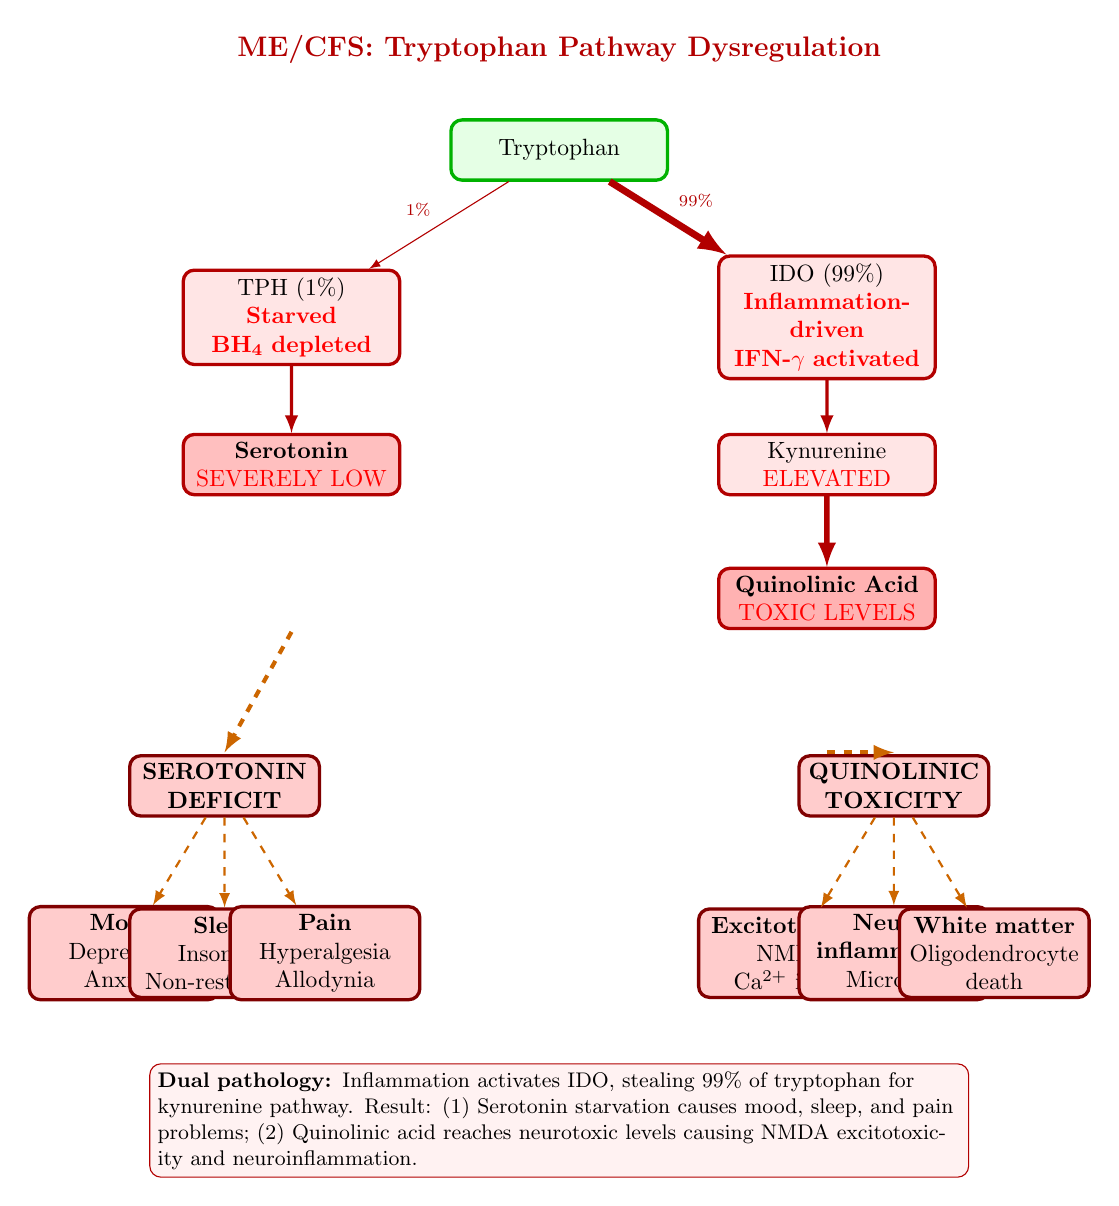
\begin{tikzpicture}[
    node distance=2.5cm,
    scale=0.85, every node/.style={scale=0.85},
    % Styles
    normal/.style={draw=green!70!black, fill=green!10, very thick, rounded corners, text width=3cm, align=center, minimum height=0.9cm},
    impaired/.style={draw=red!70!black, fill=red!10, very thick, rounded corners, text width=3cm, align=center, minimum height=0.9cm},
    pathological/.style={draw=red!50!black, fill=red!20, very thick, rounded corners, text width=2.6cm, align=center, minimum height=0.9cm},
    arrow/.style={-latex, very thick, green!70!black},
    impaired-arrow/.style={-latex, very thick, red!70!black},
    cascade-arrow/.style={-latex, thick, orange!80!black, dashed},
    note/.style={font=\scriptsize\itshape, text width=2.3cm, align=center},
]

% Title
\node[font=\large\bfseries, red!70!black] at (0, 9) {ME/CFS: Tryptophan Pathway Dysregulation};

% TOP: Dysregulated pathway
\begin{scope}[yshift=5cm]
    % Tryptophan
    \node[normal] (trp) at (0, 2.5) {Tryptophan};

    % LEFT: Serotonin - STARVED
    \node[impaired] (tph) at (-4, 0) {TPH (1\%)\\{\color{red}\textbf{Starved}}\\{\color{red}\textbf{BH\textsubscript{4} depleted}}};
    \draw[impaired-arrow, thin] (trp) -- node[above left, font=\scriptsize] {1\%} (tph);

    \node[impaired, fill=red!25] (serotonin) at (-4, -2.2) {\textbf{Serotonin}\\{\color{red}SEVERELY LOW}};
    \draw[impaired-arrow] (tph) -- (serotonin);

    % RIGHT: Kynurenine - HYPERACTIVE
    \node[impaired] (ido) at (4, 0) {IDO (99\%)\\{\color{red}\textbf{Inflammation-driven}}\\{\color{red}\textbf{IFN-$\gamma$ activated}}};
    \draw[impaired-arrow, line width=2.5pt] (trp) -- node[above right, font=\scriptsize] {99\%} (ido);

    \node[impaired] (kyn) at (4, -2.2) {Kynurenine\\{\color{red}ELEVATED}};
    \draw[impaired-arrow] (ido) -- (kyn);

    % Quinolinic acid - TOXIC
    \node[impaired, fill=red!30] (quin) at (4, -4.2) {\textbf{Quinolinic Acid}\\{\color{red}TOXIC LEVELS}};
    \draw[impaired-arrow, line width=2pt] (kyn) -- (quin);
\end{scope}

% BOTTOM: Dual pathology consequences
\begin{scope}[yshift=-4cm]
    % Serotonin deficit consequences (left)
    \node[pathological] (sero-def) at (-5, 2) {\textbf{SEROTONIN}\\  \textbf{DEFICIT}};

    \node[pathological] (mood) at (-6.5, -0.5) {\textbf{Mood}\\Depression\\Anxiety};
    \node[pathological] (sleep) at (-5, -0.5) {\textbf{Sleep}\\Insomnia\\Non-restorative};
    \node[pathological] (pain) at (-3.5, -0.5) {\textbf{Pain}\\Hyperalgesia\\Allodynia};

    \draw[cascade-arrow] (sero-def) -- (mood);
    \draw[cascade-arrow] (sero-def) -- (sleep);
    \draw[cascade-arrow] (sero-def) -- (pain);

    % Quinolinic acid consequences (right)
    \node[pathological] (quin-tox) at (5, 2) {\textbf{QUINOLINIC}\\  \textbf{TOXICITY}};

    \node[pathological] (excito) at (3.5, -0.5) {\textbf{Excitotoxicity}\\NMDA\\Ca\textsuperscript{2+} influx};
    \node[pathological] (neuroinf) at (5, -0.5) {\textbf{Neuro-}\\  \textbf{inflammation}\\Microglia};
    \node[pathological] (white) at (6.5, -0.5) {\textbf{White matter}\\Oligodendrocyte\\death};

    \draw[cascade-arrow] (quin-tox) -- (excito);
    \draw[cascade-arrow] (quin-tox) -- (neuroinf);
    \draw[cascade-arrow] (quin-tox) -- (white);
\end{scope}

% Arrows from pathway to consequences
\draw[cascade-arrow, line width=1.5pt] (-4, 0.3) -- (-5, -1.5);
\draw[cascade-arrow, line width=1.5pt] (4, -1.5) -- (5, -1.5);

% Key point box
\node[draw=red!70!black, fill=red!5, rounded corners, text width=12cm, align=left, font=\small] at (0, -7) {
\textbf{Dual pathology:} Inflammation activates IDO, stealing 99\% of tryptophan for kynurenine pathway. Result: (1) Serotonin starvation causes mood, sleep, and pain problems; (2) Quinolinic acid reaches neurotoxic levels causing NMDA excitotoxicity and neuroinflammation.
};

\end{tikzpicture}
\caption{ME/CFS tryptophan dysregulation causing serotonin deficit and quinolinic acid toxicity.}
\label{fig:tryptophan-mecfs}
\end{figure}


Figures~\ref{fig:tryptophan-normal} and~\ref{fig:tryptophan-mecfs} illustrate tryptophan metabolism dysregulation in ME/CFS. While normally approximately 95\% of tryptophan is metabolized via the kynurenine pathway, inflammation-driven IDO overactivation can substantially increase this proportion. If kynurenine pathway flux increases to approximately 99\% (a plausible estimate based on the magnitude of IDO upregulation observed in inflammatory conditions), this seemingly modest 4 percentage-point shift would dramatically reduce serotonin-available tryptophan from 5\% to 1\%---an 80\% reduction in serotonin precursor availability---while quinolinic acid accumulation reaches toxic levels.

\paragraph{Serotonin Synthesis}
Diversion of tryptophan into the kynurenine pathway reduces availability for serotonin synthesis. This 80\% reduction in available tryptophan for the serotonin pathway may contribute to sleep disturbances, mood symptoms, pain amplification, and cognitive impairment observed in ME/CFS.

\subsubsection{Serotonergic Dysfunction}

Beyond tryptophan diversion, multiple lines of evidence suggest primary serotonergic abnormalities in ME/CFS. These include altered serotonin transporter binding on PET imaging, abnormal responses to serotonergic challenge tests, correlations between serotonin markers and fatigue severity, and variable responses to serotonergic medications.

The serotonergic system's role in regulating sleep, mood, pain perception, and autonomic function makes it a plausible contributor to the multisystem dysfunction of ME/CFS.

\subsubsection{Dopaminergic Dysfunction}

Dopamine abnormalities extend beyond the CSF findings to include reduced dopamine transporter availability in basal ganglia, altered reward processing on functional imaging, blunted dopamine release in response to rewards, and correlation between dopamine markers and motivational symptoms.

The overlap between ME/CFS fatigue and the fatigue observed in Parkinson's disease and other dopaminergic disorders supports a common underlying mechanism.

\subsubsection{Norepinephrine and the Locus Coeruleus}

The locus coeruleus (LC), the primary source of brain norepinephrine, plays critical roles in arousal and sleep-wake regulation, attention and cognitive flexibility, stress responses, and autonomic nervous system modulation.

LC dysfunction could explain the constellation of arousal, attention, and autonomic abnormalities in ME/CFS. Potential mechanisms include neuroinflammation affecting LC neurons, autoantibodies targeting adrenergic receptors, metabolic stress impairing catecholamine synthesis, and chronic stress-induced LC dysregulation.

\subsubsection{GABAergic and Glutamatergic Imbalance}

Magnetic resonance spectroscopy (MRS) studies have revealed abnormalities in the balance between inhibitory (GABA) and excitatory (glutamate) neurotransmission in ME/CFS. These include elevated glutamate/glutamine in some brain regions, reduced GABA concentrations in others, altered glutamate/GABA ratios correlating with symptom severity, and regional variations in neurochemical abnormalities.

This excitatory/inhibitory imbalance could contribute to sensory hypersensitivity, cognitive dysfunction, sleep disturbances, and seizure susceptibility in some patients.

\subsubsection{Cholinergic Dysfunction}

Acetylcholine abnormalities in ME/CFS have received less attention but may contribute to cognitive impairment (particularly memory), autonomic dysfunction (parasympathetic arm), sleep architecture abnormalities, and muscle function.

Autoantibodies against muscarinic acetylcholine receptors have been identified in some ME/CFS patients, providing a potential autoimmune mechanism for cholinergic dysfunction.

\subsection{Sleep Architecture and Inter-Regional Coordination}
\label{sec:sleep-architecture}

Sleep disturbances, particularly unrefreshing sleep despite adequate duration, affect up to 95\% of ME/CFS patients. While subjective complaints are nearly universal, objective polysomnographic findings show more subtle alterations: longer sleep latency, reduced sleep efficiency, increased Stage 3 sleep in adults, and altered sleep microstructure~\cite{Jackson2023sleep}. The paradox---severe subjective sleep dysfunction with modest objective changes---suggests the problem may lie not in sleep duration or stage percentages, but in the \textit{coordination} required to generate and maintain normal sleep architecture.

\subsubsection{Energy Costs of Sleep Architecture Coordination}

Normal sleep architecture requires sophisticated inter-regional brain coordination orchestrated primarily through thalamo-cortical circuits. During non-REM sleep, slow oscillations (~1~Hz) originate in the anterior thalamus and precede neocortical slow oscillations, while sleep spindles (~12--14~Hz) detected in thalamic nuclei precede their neocortical counterparts~\cite{Fernandez2022thalamus}. This sequence---convergent cortical downstates leading thalamic downstates, which then trigger spindles projected back to cortex during the down-to-upstate transition---coordinates memory consolidation across distributed brain regions~\cite{Jiang2024ripples}.

Sleep spindle generation itself is metabolically demanding. Thalamic reticular nucleus (TRN) neurons must generate rhythmic bursts at 12--14~Hz, which requires sustained calcium channel activity, neurotransmitter synthesis and release, and coordinated inhibition of thalamocortical relay neurons. The cortex must then respond appropriately, amplifying spindles and coupling them with hippocampal ripples for memory consolidation. This inter-regional choreography demands substantial ATP and coordinated neurotransmitter systems.

Similarly, REM sleep requires brainstem activation (particularly cholinergic nuclei), thalamic relay, cortical activation approaching waking levels, and simultaneous motor inhibition via brainstem circuits. The transitions between sleep stages---requiring coordinated deactivation of one set of circuits and activation of another---may be particularly energy-intensive.

\begin{hypothesis}[Sleep Architecture Failure Hypothesis]
\label{hyp:sleep-architecture-failure}

In ME/CFS, CNS energy deficits and metabolic dysfunction prevent the sustained inter-regional coordination required for normal sleep architecture, resulting in fragmented sleep microstructure despite adequate total sleep time.

\paragraph{Mechanism.}
The hypothesis proposes that sleep architecture fragmentation in ME/CFS reflects energy-limited coordination failure:

\begin{enumerate}
    \item \textbf{Spindle generation deficit}: Thalamic reticular nucleus neurons cannot sustain the metabolic demands of rhythmic 12--14~Hz burst firing, reducing sleep spindle density and power

    \item \textbf{Slow-wave coordination failure}: Thalamo-cortical circuits cannot maintain synchronized slow oscillations across brain regions, fragmenting slow-wave sleep architecture

    \item \textbf{Stage transition impairment}: The coordinated network reconfiguration required for sleep stage transitions (more demanding than within-stage maintenance) fails preferentially, increasing sleep fragmentation

    \item \textbf{Inter-regional coherence reduction}: EEG coherence between brain regions declines during sleep, reflecting impaired functional connectivity~\cite{Sherlin2011coherence}

    \item \textbf{PEM-induced worsening}: During post-exertional malaise, when CNS energy deficits intensify, sleep architecture fragmentation worsens proportionally
\end{enumerate}

\paragraph{Supporting evidence.}
Jackson et al.~\cite{Jackson2023sleep} meta-analyzed objective sleep data from 801 adults and 477 adolescents with ME/CFS, confirming altered sleep microstructure despite the subjective-objective paradox. Adult patients showed reduced sleep efficiency, altered stage distribution (decreased Stage 2, increased Stage 3), and longer sleep latency---patterns consistent with coordination difficulties rather than simple sleep deprivation.

Sherlin et al.~\cite{Sherlin2011coherence} demonstrated that EEG spectral coherence distinguishes CFS patients from both healthy controls and depressed patients with 100\% accuracy for unmedicated CFS patients. The involvement of bilateral temporal lobes in 9 of 10 coherence factors suggests widespread inter-regional connectivity disruption, supporting the coordination failure hypothesis.

Sleep fragmentation studies show that chronic fragmentation impairs brain energy metabolism to an extent similar to total sleep deprivation, with lower glucose uptake in cortex and hippocampus~\cite{Baud2016fragmentation}. In ME/CFS, the causal arrow may reverse: primary metabolic dysfunction fragments sleep, which further worsens metabolism in a vicious cycle.

\paragraph{Testable predictions.}
\begin{enumerate}
    \item Sleep spindle density and power correlate inversely with ME/CFS symptom severity and biomarkers of CNS dysfunction
    \item Slow-wave sleep fragmentation (not just total SWS percentage) correlates with measures of metabolic dysfunction (e.g., cerebral lactate on MRS)
    \item Sleep architecture fragmentation worsens 24--72 hours post-exertion, tracking PEM time course
    \item Sleep stage transition frequency increases (shorter, more fragmented sleep stages) compared to healthy controls, even when stage percentages appear normal
    \item Inter-regional EEG coherence during sleep is reduced in ME/CFS patients, particularly in frequency bands critical for sleep oscillations (delta, sigma)
    \item Interventions improving cerebral metabolism (e.g., mitochondrial support) improve objective sleep microstructure, not just subjective sleep quality
\end{enumerate}

\paragraph{Treatment implications.}
If sleep architecture failure reflects energy-limited coordination, interventions should target: (1)~circadian optimization---maximizing sleep opportunity during the circadian nadir when sleep pressure is highest; (2)~metabolic support---mitochondrial cofactors (CoQ10, NADH) during evening hours may improve overnight cerebral metabolism~\cite{CastroMarrero2021CoQ10}; (3)~sleep stage-specific support---low-dose gabapentin or pregabalin may reduce thalamo-cortical excitability demands while supporting spindle generation; (4)~glymphatic enhancement---sleep position (lateral decubitus), avoiding late caffeine, and sleep continuity strategies; (5)~pacing-sleep integration---recognizing that sleep quality worsens predictably during PEM can guide activity management.

\paragraph{Limitations.}
This hypothesis has moderate certainty (0.50). No published studies have quantified spindle density or power in ME/CFS with simultaneous metabolic measures. Coherence data exists for waking but not sleep EEG. Alternative explanations include primary brainstem pathology, autonomic dysfunction, or circadian disruption rather than energy limitation. Causality direction remains unclear: does poor metabolism fragment sleep, or does fragmented sleep worsen metabolism?
\end{hypothesis}

\subsection{Glial Cell Dysfunction}
\label{sec:glial}

Beyond neurons and neurotransmitters, glial cells play critical support roles in brain function. Dysfunction in these cells may contribute to the neuroinflammation mentioned in catecholamine synthesis impairment and broader CNS pathology.

\subsubsection{Microglial Activation and Neuroinflammation}

Microglia, the resident immune cells of the central nervous system, have emerged as key players in ME/CFS neuroinflammation. Evidence for microglial activation includes elevated markers in CSF (soluble CD14, chitotriosidase), PET imaging showing increased translocator protein (TSPO) binding in specific brain regions~\cite{Nakatomi2014neuroinflammation}, correlation between neuroinflammatory markers and symptom severity, and persistence of microglial activation years after initial infection.

\textbf{Important note on replication:} The Nakatomi et al.\ 2014 study documenting widespread microglial activation via PET imaging in ME/CFS patients has not been consistently replicated, with later studies showing conflicting results. The certainty of microglial activation as a universal feature of ME/CFS remains medium pending further replication studies.

Chronic microglial activation, when present, can produce sustained release of pro-inflammatory cytokines (IL-1$\beta$, TNF-$\alpha$, IL-6), oxidative stress through reactive oxygen species production, glutamate release contributing to excitotoxicity, disruption of synaptic pruning and plasticity, and blood-brain barrier dysfunction.

\begin{hypothesis}[Glial Maturation Window and Pediatric Recovery]
\label{hyp:glial-maturation-window}

Adolescent ME/CFS patients may benefit from a developmental window during which active microglial remodeling can reset pathological activation states---a mechanism unavailable to adult patients whose glial maturation is complete.

\paragraph{Background: Adolescent Microglial Maturation}

Microglia undergo dramatic functional reorganization during adolescence, performing complex developmental tasks beyond their immune surveillance role. From embryonic neuronal migration to adolescent circuit refinement, immune signaling molecules serve as a common language allowing microglia to modulate brain function in both health and disease~\cite{Dziabis2022microglia}.

Three critical periods define microglial contributions to neural development: embryonic wiring, early postnatal synaptic pruning (peak near birth continuing into late-20s), and adolescent circuit refinement~\cite{Dziabis2022microglia}. During adolescence specifically, microglia mediate experience-dependent synaptic pruning through complement-mediated mechanisms, with C3 binding to CR3 receptors facilitating selective synapse elimination. This process exhibits sex-specific patterns and regional variation, with particularly robust activity in prefrontal cortex and nucleus accumbens~\cite{ScienceAdvances2024adolescent,PMC11758907synapse}.

Crucially, transient microglial deficiency during adolescence---but not adulthood---produces lasting cognitive impairments, identifying adolescence as a sensitive period for prefrontal microglia to act on cognitive development~\cite{ScienceAdvances2024adolescent}. The developmental program requires coordinated microglial activity for proper circuit maturation, with major transitions largely complete by early 20s.

\paragraph{Application to ME/CFS: The Reset Hypothesis}

If ME/CFS involves chronic microglial activation locked in a pro-inflammatory state (as suggested by Nakatomi et al.\ PET findings~\cite{Nakatomi2014neuroinflammation}), then adolescent microglial remodeling may provide a natural mechanism for resolution:

\begin{enumerate}
    \item \textbf{Active turnover}: Adolescent microglia undergo programmed replacement and phenotypic switching as part of circuit refinement, potentially eliminating pathologically activated cells

    \item \textbf{Developmental override signals}: The hormonal and neurochemical milieu of adolescence (BDNF elevation, sex hormones, growth factors) provides strong pro-plasticity signals that may override inflammatory set-points

    \item \textbf{Synaptic reorganization}: Pathological neuroinflammatory states often involve aberrant synaptic connections; adolescent pruning may eliminate these circuits while preserving functional connectivity

    \item \textbf{Adult lock-in}: After developmental windows close (~age 25), microglia lose plasticity for wholesale phenotypic switching, becoming locked in their current activation state without the developmental cues that enable adolescent reset
\end{enumerate}

This framework explains why pediatric ME/CFS shows substantially higher recovery rates (estimated 54--94\% in studies of mild-moderate cases) compared to adult-onset disease where recovery is rare~\cite{Rowe2019pediatric}. The critical variable is not disease duration but rather whether onset occurs before or after completion of microglial maturation.

\paragraph{Testable Predictions}

This hypothesis generates specific, falsifiable predictions:

\begin{enumerate}
    \item \textbf{Age-dependent neuroinflammation}: Longitudinal PET imaging should show declining microglial activation in recovering adolescents but persistent activation in adults with similar disease duration

    \item \textbf{Transition age threshold}: Recovery rates should decline sharply around age 22--25 (completion of prefrontal maturation) rather than showing gradual age-related decline

    \item \textbf{Biomarker trajectories}: CSF inflammatory markers (sCD14, chitotriosidase) should normalize in recovering adolescents but remain elevated in non-recovering adults

    \item \textbf{Microglial turnover markers}: Adolescent patients should show elevated markers of microglial turnover (CSF1R expression, fractalkine signaling) compared to adults

    \item \textbf{Severity interactions}: Hypothesis predicts age matters less if microglial activation is mild (can resolve spontaneously) but becomes critical if activation is severe (requires active remodeling to clear)
\end{enumerate}

\paragraph{Treatment Implications}

If adolescent microglial plasticity enables recovery, then therapeutically inducing similar plasticity in adults might improve outcomes:

\begin{enumerate}
    \item \textbf{CSF-1R inhibitors}: Drugs like PLX5622 or pexidartinib force microglial turnover by depleting existing populations and promoting repopulation from progenitors. This mimics the natural turnover occurring during adolescence, potentially resetting activation states~\cite{MDPI2024microglial}.

    \item \textbf{Fasting-mimicking diets}: Prolonged fasting promotes microglial autophagy and phenotypic switching, potentially enabling transition from pro-inflammatory to surveillance phenotypes without complete depletion

    \item \textbf{BDNF enhancement}: Brain-derived neurotrophic factor drives developmental plasticity; strategies to boost BDNF (exercise within energy envelope, ketogenic diet, certain medications) may partially reopen plasticity windows

    \item \textbf{Timing considerations}: Interventions targeting microglial reset may be most effective in younger adults (under 30) where some residual developmental plasticity remains, with diminishing returns in older patients
\end{enumerate}

\paragraph{Integration with Broader ME/CFS Pathophysiology}

This hypothesis complements rather than contradicts other mechanistic proposals. Microglial activation may be downstream of initial triggers (viral infection, autoantibodies, autonomic dysfunction) while still representing a critical perpetuating factor. The developmental window hypothesis specifically addresses \emph{why recovery patterns differ by age} rather than explaining disease initiation.

The glial maturation window may interact synergistically with other proposed pediatric advantages: immune memory pruning (Hypothesis~\ref{hyp:immune-memory-pruning}, if present), greater HSC regenerative capacity, higher baseline recovery capital (Section~\ref{spec:recovery-capital}), and incomplete epigenetic aging.

\paragraph{Limitations and Uncertainties}

Several important caveats apply:

\begin{enumerate}
    \item The Nakatomi et al.\ microglial activation findings have not been consistently replicated; if microglial activation is not a universal ME/CFS feature, this hypothesis applies only to a subset

    \item The proposed mechanism assumes glial maturation windows close around age 25, but individual variation exists; some adults may retain plasticity longer

    \item Pediatric recovery may reflect multiple mechanisms simultaneously; isolating the specific contribution of microglial remodeling requires longitudinal studies with neuroimaging

    \item CSF-1R inhibitor strategies carry significant risks (meningitis, visual changes) and remain experimental; safety in ME/CFS populations is unknown
\end{enumerate}

\paragraph{Research Priorities}

To test this hypothesis rigorously:

\begin{enumerate}
    \item \textbf{Age-stratified longitudinal neuroimaging}: Serial PET scans in adolescent vs adult ME/CFS tracking microglial activation trajectories over 2--5 years

    \item \textbf{CSF biomarker studies}: Compare inflammatory markers and microglial turnover signatures across age groups and recovery status

    \item \textbf{Preclinical models}: Post-viral fatigue models in adolescent vs adult mice to test whether developmental microglia enable recovery

    \item \textbf{Treatment trials}: Small pilot studies of CSF-1R modulation in carefully selected adult ME/CFS patients with documented microglial activation
\end{enumerate}

This hypothesis provides a mechanistic framework for understanding one component of the pediatric recovery advantage while suggesting potential therapeutic strategies for adult patients.

\end{hypothesis}

\subsubsection{Astrocyte Abnormalities and the Astrocyte Energy Gate}
\label{sec:astrocyte-energy-gate}

Astrocytes perform essential functions including neurotransmitter uptake and recycling, blood-brain barrier maintenance, metabolic support for neurons, synaptic modulation, and ion homeostasis. Astrocyte dysfunction in ME/CFS may contribute to impaired glutamate clearance and excitotoxicity, reduced metabolic support for neurons, blood-brain barrier compromise, and abnormal synaptic transmission. Elevated GFAP (glial fibrillary acidic protein) in some ME/CFS patients suggests astrocyte reactivity, though findings have been inconsistent.

Beyond these recognized roles, astrocytes occupy a uniquely critical position in brain energy metabolism that may constitute a central vulnerability in ME/CFS. The following hypothesis develops this metabolic dimension in detail.

\paragraph{The Astrocyte-Neuron Lactate Shuttle: Normal Physiology}

The brain consumes 20--25\% of the body's glucose despite comprising only 2\% of body mass~\cite{Belanger2011}. A substantial fraction of this energy reaches neurons not as glucose directly, but via the \textbf{astrocyte-neuron lactate shuttle} (ANLS), first described by Pellerin and Magistretti~\cite{Pellerin1994}. In this system, glutamate released during synaptic transmission is taken up by astrocytes via excitatory amino acid transporters (EAATs), triggering astrocytic glucose uptake through GLUT1 transporters and subsequent glycolysis. Astrocytes convert glucose to pyruvate and then to lactate via lactate dehydrogenase A (LDHA), which preferentially catalyzes the pyruvate-to-lactate direction. This lactate is then exported from astrocytes through monocarboxylate transporter 4 (MCT4, a low-affinity, high-capacity exporter) and imported into neurons through MCT2 (a high-affinity importer)~\cite{Pierre2005}. Within neurons, LDHB converts lactate back to pyruvate for oxidative phosphorylation in mitochondria.

This architecture elegantly couples neuronal energy supply to neuronal activity: when a synapse fires, the glutamate released simultaneously signals the local astrocyte to increase energy delivery~\cite{Magistretti2018}. Lactate provides an estimated 30--50\% of neuronal ATP under physiological conditions~\cite{Magistretti2018}, and this fraction likely increases during periods of intense neural activity when neurons' own glycolytic capacity is insufficient.

Several features make this shuttle critical rather than merely supplementary:

\begin{enumerate}
    \item \textbf{Activity coupling:} The glutamate-triggered mechanism ensures energy supply scales with demand at the single-synapse level
    \item \textbf{Metabolic specialization:} Neurons preferentially express LDHB (favoring lactate $\to$ pyruvate) while astrocytes express LDHA (favoring pyruvate $\to$ lactate), creating directional metabolic flow~\cite{Kim2025ANLS}
    \item \textbf{Antioxidant protection:} By outsourcing glycolysis to astrocytes, neurons can direct more glucose through the pentose phosphate pathway for glutathione regeneration, protecting against oxidative damage
    \item \textbf{Signaling function:} Lactate also acts as a signaling molecule via the hydroxycarboxylic acid receptor 1 (HCAR1/GPR81), modulating neuronal excitability and synaptic plasticity~\cite{Magistretti2018}
\end{enumerate}

\paragraph{Important Nuance: Neuronal Metabolic Flexibility}

The classical ANLS model has been refined by recent evidence demonstrating that neurons possess greater metabolic flexibility than originally assumed. Single-cell RNA sequencing studies reveal that neurons express both LDHA and LDHB, not exclusively LDHB~\cite{Kim2025ANLS}. Neurons can directly take up and oxidize glucose, particularly during high-demand states. LDHB-deficient neurons maintain stable energy metabolism under physiological glucose conditions, suggesting compensatory pathways exist.

However, this flexibility has limits. During high-frequency neural activity---precisely the conditions of cognitive exertion---direct neuronal glucose oxidation may prove insufficient, and astrocyte-derived lactate becomes the critical marginal fuel source. This distinction between \emph{basal} sufficiency and \emph{demand-responsive} insufficiency is central to the hypothesis that follows.

\begin{hypothesis}[Astrocyte Energy Gate]
\label{hyp:astrocyte-energy-gate}
We hypothesize that dysfunction in the astrocyte-neuron lactate shuttle creates a \textbf{metabolic bottleneck}---an ``energy gate''---that produces CNS-specific energy failure in ME/CFS while peripheral tissues with direct glucose access remain unaffected.

\paragraph{Three Candidate Mechanisms}

The energy gate may fail at any of three nodes, singly or in combination:

\begin{enumerate}
    \item \textbf{Astrocyte glucose uptake impairment (GLUT1 dysfunction):} Reduced GLUT1 expression or function on astrocytes limits the raw substrate entering the shuttle. GLUT1 deficiency syndrome demonstrates that impaired astrocytic glucose transport causes seizures, cognitive impairment, and brain hypometabolism---features that partially overlap with ME/CFS neurological symptoms. Neuroinflammatory mediators (IL-1$\beta$, TNF-$\alpha$) documented in ME/CFS can downregulate GLUT1 expression.

    \item \textbf{Lactate production impairment (glycolytic defects):} Reactive astrogliosis---documented via elevated GFAP in ME/CFS---involves metabolic reprogramming that may paradoxically impair effective lactate delivery. While reactive astrocytes initially upregulate glycolysis, chronic neuroinflammation shifts astrocyte metabolism toward a state where mitochondrial dysfunction reduces overall metabolic efficiency. Inflammatory cytokines can alter pyruvate dehydrogenase kinase (PDK) activity, disrupting the glycolysis/oxidative phosphorylation balance within astrocytes themselves.

    \item \textbf{Lactate transport impairment (MCT dysfunction):} Downregulation of MCT4 (astrocyte export) or MCT2 (neuronal import) directly restricts lactate flow. This mechanism has the strongest precedent in other neurological diseases: MCT1/MCT4 downregulation reduces neuronal lactate supply by approximately 60\%~\cite{Kim2025ANLS}. In Alzheimer's disease, decreased expression of MCT1, MCT2, and MCT4 is documented. In amyotrophic lateral sclerosis, reduced MCT1 in oligodendrocytes precedes motor neuron degeneration. In temporal lobe epilepsy, MCT2 redistribution and MCT4 reduction are observed in epileptic foci.
\end{enumerate}

\paragraph{Why This Creates Selective Dysfunction}

The energy gate hypothesis explains why CNS function fails while peripheral tissues remain functional:

\begin{itemize}
    \item \textbf{CNS vulnerability:} Neurons depend on the ANLS for a substantial portion of their activity-dependent energy supply. No other cell type in the body has this intermediary requirement for its primary fuel.
    \item \textbf{Peripheral independence:} Skeletal muscle, cardiac muscle, and peripheral tissues express GLUT4 (insulin-responsive) and can directly oxidize glucose without astrocytic intermediation. Hair follicles operate autonomous local Cori cycles, recycling lactate within the follicular unit without CNS coordination.
    \item \textbf{Demand-dependence:} The ANLS is most critical during cognitive exertion (when glutamate release surges trigger proportional lactate demand). This explains why cognitive symptoms worsen with mental effort while resting cognition may remain closer to normal---a hallmark of ME/CFS ``brain fog.''
\end{itemize}

This mechanism connects directly to the selective energy dysfunction hypothesis (Section~\ref{sec:selective-dysfunction}), which predicts that high CNS-dependency ($\alpha$) and high demand-responsiveness ($\rho$) processes should be most impaired. The ANLS provides the \emph{specific molecular mechanism} through which this selective vulnerability operates.

\paragraph{Certainty Assessment}

This hypothesis integrates well-established neuroscience (ANLS physiology: high certainty) with speculative application to ME/CFS (low-to-moderate certainty). No study has directly measured ANLS flux, MCT expression, or astrocyte-specific glycolytic rates in ME/CFS patients. The hypothesis is graded at \textbf{certainty 0.35}: mechanistically plausible, consistent with indirect evidence, but requiring direct experimental validation.
\end{hypothesis}

\paragraph{Supporting Evidence: Brain Lactate Elevation}

While no study has directly assayed ANLS function in ME/CFS, magnetic resonance spectroscopy (MRS) studies provide indirect evidence consistent with impaired brain energy metabolism:

\begin{itemize}
    \item \textbf{7T MRS (2025):} Godlewska et al.~\cite{Godlewska2025MRS} found elevated lactate in the pregenual anterior cingulate cortex (pgACC: 1.52 vs.\ 1.22~mM, $p = 0.003$) and dorsal ACC (dACC) of ME/CFS patients (n=24) compared to healthy controls (n=24), using ultra-high-field 7 Tesla MRS. Notably, ME/CFS and Long COVID patients showed \emph{different} neurochemical profiles despite similar clinical presentations.

    \item \textbf{Whole-brain MRS (2020):} Mueller et al.~\cite{Mueller2020MRS} documented elevated lactate-to-creatine ratios in the right insula, thalamus, and cerebellum (n=15 ME/CFS vs.\ n=15 controls), with brain temperature increases correlated with lactate elevations---suggesting neuroinflammation drives metabolic shifts.

    \item \textbf{Mitochondrial review (2025):} Syed et al.~\cite{Syed2025MitoCFS} synthesize evidence of elevated CSF lactate, impaired ATP synthesis, and increased glycolytic activity in ME/CFS, consistent with oxidative stress and conditions favoring anaerobic metabolism.
\end{itemize}

\begin{warning}[Interpreting Elevated Brain Lactate]
Elevated brain lactate in ME/CFS is consistent with the energy gate hypothesis but does not uniquely support it. At least three interpretations are possible:
\begin{enumerate}
    \item \textbf{ANLS dysfunction:} Lactate accumulates in astrocytes because it cannot be efficiently exported to or utilized by neurons (supports the energy gate hypothesis)
    \item \textbf{Mitochondrial dysfunction:} Neuronal mitochondria cannot oxidize lactate efficiently, causing backpressure (supports a downstream mitochondrial hypothesis)
    \item \textbf{Anaerobic shift:} Increased glycolysis due to hypoperfusion or oxygen limitation produces excess lactate (supports a vascular hypothesis)
\end{enumerate}
These mechanisms are not mutually exclusive and may operate simultaneously. Distinguishing between them requires studies that measure not just lactate levels but lactate \emph{flux} between cellular compartments---technically challenging but feasible with advanced $^{13}$C-MRS techniques.
\end{warning}

\paragraph{Testable Predictions}

The astrocyte energy gate hypothesis generates specific, falsifiable predictions that distinguish it from alternative explanations:

\begin{enumerate}
    \item \textbf{CSF lactate gradient:} If astrocytes produce lactate but neurons cannot utilize it, the CSF lactate/blood lactate ratio should be elevated in ME/CFS (astrocyte-derived lactate accumulating in extracellular space). In mitochondrial disorders affecting the CNS, a CSF/blood lactate ratio $> 0.91$ indicates central origin~\cite{Syed2025MitoCFS}. \\
    \emph{Prediction:} ME/CFS patients will show CSF/blood lactate ratio $> 0.91$, distinguishing CNS-origin lactate from peripheral sources.

    \item \textbf{MCT expression profiling:} Post-mortem or biopsy studies should reveal reduced MCT2 (neuronal) and/or MCT4 (astrocyte) expression in ME/CFS brain tissue, particularly in regions showing functional deficits (prefrontal cortex, anterior cingulate). \\
    \emph{Prediction:} MCT2/MCT4 expression reduced $\geq$30\% vs.\ matched controls.

    \item \textbf{Astrocyte-specific metabolomics:} Single-cell or spatial transcriptomics of ME/CFS brain tissue should show altered expression of glycolytic enzymes (hexokinase, phosphofructokinase, LDHA) and glucose transporters (GLUT1) in astrocytes specifically. \\
    \emph{Prediction:} Astrocyte glycolytic gene expression altered while neuronal oxidative genes remain intact.

    \item \textbf{Exogenous lactate challenge:} If the bottleneck is at the glucose $\to$ lactate step (mechanisms 1 or 2 above), then providing exogenous lactate should partially bypass the gate and improve cognitive function. If the bottleneck is at MCT transport (mechanism 3), exogenous lactate should not help. \\
    \emph{Prediction:} IV sodium lactate infusion during cognitive testing will improve performance in a subgroup of ME/CFS patients.

    \item \textbf{Ketone body bypass:} Ketone bodies ($\beta$-hydroxybutyrate, acetoacetate) enter neurons via MCT2 and are metabolized directly in neuronal mitochondria, bypassing the astrocyte glycolysis step entirely~\cite{Jang2024Ketone}. If the energy gate is at the astrocyte level, ketones should preferentially benefit CNS symptoms. \\
    \emph{Prediction:} Ketogenic diet or exogenous ketone supplementation will improve cognitive symptoms disproportionately to peripheral fatigue symptoms.

    \item \textbf{Activity-dependent worsening:} Since the ANLS is most critical during high neural activity (when glutamate-triggered demand surges), the energy gate should cause greater deficits during cognitive exertion than at rest. \\
    \emph{Prediction:} The difference between resting and task-evoked brain lactate (measured by functional MRS) will be larger in ME/CFS than controls---reflecting both increased demand signaling and impaired supply response.
\end{enumerate}

\paragraph{Treatment Implications}

The energy gate framework suggests several therapeutic strategies, ordered by plausibility and feasibility:

\begin{enumerate}
    \item \textbf{Ketogenic diet or exogenous ketones:} By providing $\beta$-hydroxybutyrate directly to neurons via MCT2, this approach bypasses the astrocyte glycolysis step entirely. The ketogenic diet has established neuroprotective effects in epilepsy (where MCT dysfunction is documented) and emerging evidence in psychiatric disorders associated with brain energy dysfunction~\cite{Jang2024Ketone}. \emph{This represents the most immediately testable intervention.}

    \item \textbf{Exogenous lactate supplementation:} Sodium lactate infusion or oral lactate has shown cognitive benefits in Alzheimer's disease models by restoring hippocampal and CSF lactate concentrations. In ME/CFS, this could bypass impaired astrocyte glycolysis (mechanisms 1--2) but would not help if MCT2 transport is the bottleneck (mechanism 3).

    \item \textbf{MCT upregulation:} Exercise and certain pharmacological agents can upregulate MCT expression. However, exercise intolerance in ME/CFS limits this approach. Pharmacological MCT modulators remain experimental.

    \item \textbf{Anti-neuroinflammatory strategies:} If chronic neuroinflammation drives astrocyte metabolic reprogramming and MCT downregulation, targeting neuroinflammation at its source may restore ANLS function. Low-dose naltrexone (LDN), which modulates microglial activation, could theoretically improve astrocyte metabolic function through reduced neuroinflammatory signaling.

    \item \textbf{Astrocyte-targeted delivery:} Emerging drug delivery technologies using astrocyte-specific targeting (e.g., nanoparticles with GFAP-binding peptides) could deliver metabolic support directly to astrocytes, enhancing glycolytic capacity or MCT expression without systemic effects.
\end{enumerate}

\paragraph{Limitations and Alternative Explanations}

Several important caveats apply to this hypothesis:

\begin{itemize}
    \item \textbf{No direct evidence in ME/CFS:} No study has measured ANLS flux, MCT expression, or astrocyte-specific glycolytic rates in ME/CFS patients. The hypothesis rests entirely on indirect evidence (elevated brain lactate, documented neuroinflammation) and analogy to other neurological conditions.

    \item \textbf{Elevated lactate is ambiguous:} As noted above, elevated brain lactate has at least three interpretations. The ANLS dysfunction interpretation is not uniquely supported by current data.

    \item \textbf{The ANLS itself is debated:} While the ANLS is well-established, its quantitative contribution remains contested. Some evidence suggests neurons can sustain activity through direct glucose oxidation alone, at least under non-demanding conditions~\cite{Kim2025ANLS}. The hypothesis is strongest for high-demand cognitive states.

    \item \textbf{Downstream mitochondrial dysfunction:} Even if lactate reaches neurons normally, impaired neuronal mitochondria (a well-documented finding in ME/CFS~\cite{Syed2025MitoCFS}) would produce similar symptoms. The energy gate and mitochondrial hypotheses are not mutually exclusive but have different treatment implications.

    \item \textbf{GLUT1 paradox:} Recent studies show that astrocyte-specific GLUT1 reduction can \emph{paradoxically improve} brain glucose metabolism, suggesting compensatory mechanisms may complicate predictions based on simple GLUT1 downregulation.

    \item \textbf{Small sample sizes:} The MRS studies supporting brain lactate elevation in ME/CFS have samples of n=15--24, which limits statistical power and generalizability. Larger, multi-site replication studies are needed.
\end{itemize}

For the relationship between the astrocyte energy gate and the broader selective energy dysfunction framework, including formal mathematical treatment and additional predictions, see Section~\ref{sec:selective-dysfunction}, specifically the astrocyte energy gate sub-hypothesis~(\ref{hyp:astrocyte-gate}).

\subsubsection{Oligodendrocyte Function}

Oligodendrocytes produce the myelin sheaths essential for rapid nerve conduction. Potential abnormalities include demyelination contributing to white matter hyperintensities, impaired remyelination capacity, oxidative damage to oligodendrocytes, and disrupted axon-glial signaling.

The white matter changes observed on MRI in ME/CFS patients may reflect oligodendrocyte dysfunction, though the mechanisms remain to be fully elucidated.

\subsubsection{Developmental Context: The Glial Maturation Window}

The discussion of microglial activation in ME/CFS has largely overlooked a critical developmental dimension: the adolescent brain undergoes dramatic microglial reorganization that may explain the differential recovery rates between pediatric and adult patients.

\begin{speculation}[Glial Maturation Window]
\label{spec:glial-maturation}
We propose that adolescent developmental neuroplasticity includes a ``glial maturation window'' during which microglial populations undergo programmed reprogramming that can reset aberrant activation states. This window may explain why pediatric ME/CFS patients recover at dramatically higher rates than adults despite similar initial neuroinflammatory pathology.

\paragraph{Developmental Neuroscience Foundation}
Microglia are not static cells; they undergo profound changes during brain development. During adolescence, several coordinated processes occur:

\textit{Synaptic pruning intensification.} The adolescent brain eliminates approximately 50\% of synapses through microglia-mediated pruning, refining neural circuits~\cite{Paolicelli2011synaptic}. This process peaks around puberty and extends into the early twenties. The pruning machinery requires microglia to transition between surveillance and phagocytic states repeatedly.

\textit{Microglial reprogramming.} As pruning completes, microglia must reset from active phagocytic states to homeostatic surveillance. This reprogramming involves transcriptional reorganization, morphological changes, and functional recalibration. Developmental signals (CSF-1, IL-34, TGF-$\beta$) coordinate this transition.

\textit{Complement system maturation.} The complement cascade (C1q, C3) tags synapses for elimination during development. Complement expression declines after the pruning window closes, potentially reducing the brain's capacity for similar reorganization in adulthood.

\paragraph{Hypothesis: Developmental Pruning Resets Neuroinflammation}
If ME/CFS triggers chronic microglial activation (as suggested by Nakatomi et al.'s PET data, pending replication), adolescent patients may have an inherent advantage: the ongoing developmental pruning program could ``sweep away'' aberrantly activated microglia along with the synapses being eliminated. The same signals that coordinate normal developmental pruning may force activated microglia to either reset to surveillance phenotypes or be replaced by newly differentiated cells from progenitor pools.

In adults, this developmental program is complete. Microglia that shift to pro-inflammatory phenotypes lack the developmental signals that would trigger reset. Without external intervention, activated microglia may persist indefinitely, maintaining chronic neuroinflammation.

\paragraph{Testable Predictions}
This hypothesis generates several falsifiable predictions:
\begin{enumerate}
    \item PET imaging with TSPO ligands should show higher microglial activation in adult ME/CFS patients compared to pediatric patients of similar disease duration and severity.
    \item Pediatric ME/CFS patients who recover should show normalization of microglial markers over time, while non-recovering patients (and adults) should show persistent activation.
    \item The recovery rate differential should diminish for patients whose onset occurs after the developmental window closes (early twenties).
    \item Biomarkers of developmental pruning activity (complement proteins, synaptic markers in CSF) should correlate with recovery probability in pediatric patients.
\end{enumerate}

\paragraph{Therapeutic Implications}
If the glial maturation window hypothesis is correct, therapeutic strategies could aim to artificially induce microglial turnover or reprogramming in adults:

\textit{CSF-1R inhibition.} Colony-stimulating factor 1 receptor (CSF-1R) is essential for microglial survival. CSF-1R inhibitors (such as PLX5622 in animal models, or pexidartinib which is FDA-approved for tenosynovial giant cell tumors) can deplete microglia, which then repopulate from CNS progenitors in a potentially ``reset'' state. Preclinical studies in mouse models of neuroinflammation show that microglial depletion and repopulation can resolve chronic neuroinflammatory states~\cite{Elmore2014csf1r}. However, global microglial depletion carries risks, and clinical translation for ME/CFS would require careful safety evaluation.

\textit{Fasting-mimicking interventions.} Prolonged fasting or fasting-mimicking diets have been shown to promote microglial turnover and reduce neuroinflammation in animal models~\cite{Choi2018fasting}. The mechanisms may involve autophagy induction, stem cell activation, and metabolic reprogramming. While speculative for ME/CFS, dietary interventions represent a lower-risk approach to test the hypothesis.

\textit{BDNF and neuroplasticity promoters.} Brain-derived neurotrophic factor (BDNF) promotes neural plasticity and may influence microglial phenotype. Interventions that increase BDNF (exercise in those who tolerate it, certain antidepressants, photobiomodulation) could theoretically support glial homeostasis, though evidence in ME/CFS is limited.

\paragraph{Research Priorities}
Priority research to test this hypothesis should include:
\begin{enumerate}
    \item Comparative PET neuroimaging study of pediatric versus adult ME/CFS patients using second-generation TSPO ligands
    \item Longitudinal CSF biomarker study tracking microglial activation markers (sTREM2, chitotriosidase) in pediatric patients through recovery or chronification
    \item Preclinical studies of CSF-1R inhibition in post-viral fatigue animal models
    \item Safety and feasibility studies of fasting-mimicking protocols in stable ME/CFS patients
\end{enumerate}

\paragraph{Limitations}
This hypothesis rests on uncertain foundations. The Nakatomi et al.\ PET findings require replication. The developmental neuroscience of microglial reprogramming is still being elucidated, and translation from animal models to human disease is uncertain. The hypothesis also does not explain why some pediatric patients fail to recover, though this could reflect variation in the timing or completeness of developmental processes.

Despite these limitations, the glial maturation window hypothesis provides a testable framework for understanding the pediatric recovery advantage through a neuroimmune lens. If supported by evidence, it would suggest specific therapeutic targets for inducing microglial reset in adult patients. A comparative study of pediatric versus adult ME/CFS patients (Section~\ref{sec:pediatric-adult-study}) could help test predictions of this hypothesis.
\end{speculation}

\subsubsection{Post-Viral CNS Reprogramming}

The preceding sections document microglial activation, astrocyte dysfunction, and neuroinflammatory cascades in ME/CFS. A critical question is why these states persist long after the triggering infection resolves. Emerging evidence from trained immunity research suggests that a single viral infection can permanently alter glial cell function through epigenetic mechanisms.

\begin{speculation}[Post-Viral CNS Reprogramming Hypothesis]
\label{spec:post-viral-cns-reprogramming}

Viral infection causes persistent epigenetic reprogramming of astrocytes and microglia, creating a lasting shift in CNS metabolism that persists long after viral clearance. This mechanism---analogous to ``trained immunity'' in peripheral innate immune cells---may explain why ME/CFS becomes chronic following acute infection.

\paragraph{Trained immunity and epigenetic memory.}
Trained immunity refers to the capacity of innate immune cells to develop long-lasting functional memory following initial stimulation~\cite{Humer2025TrainedImmunityMECFS}. Unlike adaptive immune memory mediated by lymphocyte clonal expansion, trained immunity operates through persistent epigenetic modifications---particularly histone marks such as H3K4me1 and H3K27ac at inflammatory gene promoters---that prime cells for enhanced responses to subsequent stimuli. Humer et al.\ advocate trained immunity as a contributing factor to ME/CFS pathogenesis, proposing that post-infectious epigenetic reprogramming of innate immune cells produces a hyperresponsive phenotype that sustains chronic inflammation~\cite{Humer2025TrainedImmunityMECFS}.

\paragraph{Microglial epigenetic reprogramming.}
Wendeln et al.\ demonstrated in a landmark \textit{Nature} study that peripheral inflammatory stimuli induce long-lasting epigenetic reprogramming of brain microglia~\cite{Wendeln2018InnateImmuneMemoryBrain}. Trained microglia develop enhanced H3K4me1 marks at inflammatory gene loci that persist for months after the initial stimulus and exacerbate subsequent neurological pathology. This immune memory operates through metabolic reprogramming: activated microglia shift from oxidative phosphorylation to aerobic glycolysis, and this metabolic phenotype becomes epigenetically stabilized~\cite{Nirakis2025MetabolicRegulationMicroglial}. The persistence of these marks means that a single viral infection could establish a ``new normal'' of microglial function that outlasts the infection by years.

\paragraph{Viral reprogramming of glial metabolism.}
Rodrigues et al.\ demonstrate that neurotropic viruses---including SARS-CoV-2, HIV-1, and Zika virus---directly infect astrocytes and microglia, causing metabolic shifts from oxidative phosphorylation to glycolysis with consequent NLRP3 inflammasome activation~\cite{Rodrigues2025ViralReprogrammingGlialMetabolism}. This metabolic reprogramming is not merely a transient response to active infection; it persists because the glycolytic shift triggers epigenetic modifications that stabilize the pro-inflammatory phenotype. The result is a self-sustaining cycle: viral infection $\rightarrow$ metabolic shift $\rightarrow$ epigenetic stabilization $\rightarrow$ chronic neuroinflammation.

This mechanism has direct relevance to the astrocyte energy gate hypothesis (Section~\ref{sec:astrocyte-energy-gate}): if viral infection reprograms astrocytes to favor glycolysis over oxidative phosphorylation, lactate production via the astrocyte-neuron lactate shuttle may be disrupted. Astrocytes locked in a glycolytic-inflammatory phenotype may consume glucose for their own inflammatory signaling rather than converting it to lactate for neuronal use.

\paragraph{Broader epigenetic landscape in ME/CFS.}
Apostolou and Ros\'en document over 12,000 altered CpG methylation sites in ME/CFS patients, with particular enrichment at immune and metabolic gene loci~\cite{Apostolou2024EpigeneticReprogrammingMECFS}. They propose that latent herpesviruses (particularly EBV) employ long-term epigenetic strategies that may permanently alter host cell function. Complementing this, Iu et al.\ demonstrate that CD8$^+$ T cells in ME/CFS exhibit epigenetic predisposition toward terminal exhaustion, with exhaustion markers upregulated following exercise challenge~\cite{Iu2024TranscriptionalReprogrammingCD8}---linking immune reprogramming directly to post-exertional malaise.

\paragraph{Testable predictions.}
\begin{enumerate}
    \item Post-infectious ME/CFS patients should show distinct microglial epigenetic signatures (elevated H3K4me1/H3K27ac at inflammatory loci) compared to gradual-onset patients, detectable via CSF-derived microglia or post-mortem analysis
    \item Astrocyte metabolic profiles (measurable via MRS glutamate/glutamine ratios) should differ between post-viral and non-viral ME/CFS subtypes
    \item Epigenetic modifiers targeting trained immunity (e.g., histone methyltransferase inhibitors, mTOR pathway modulators) should preferentially benefit post-infectious ME/CFS
    \item Early antiviral or anti-inflammatory intervention during acute infection should reduce ME/CFS incidence by preventing epigenetic stabilization
    \item CSF cytokine profiles should show trained immunity signatures (enhanced IL-6, TNF-$\alpha$ responses to ex vivo stimulation) in post-infectious but not gradual-onset patients
\end{enumerate}

\paragraph{Treatment implications.}
If post-viral CNS reprogramming drives chronic ME/CFS, therapeutic strategies should target epigenetic reversal rather than symptomatic suppression: (1)~epigenetic modifiers that can cross the BBB and reset microglial histone marks; (2)~metabolic interventions that shift astrocytes back from glycolysis to oxidative phosphorylation; (3)~microglial depletion and repopulation via CSF-1R inhibition (see Section~\ref{spec:glial-maturation}), which may generate microglia without the trained immunity epigenetic marks; (4)~early intervention protocols during acute viral illness to prevent epigenetic stabilization.

\paragraph{Limitations.}
This hypothesis has certainty 0.40. No study has directly measured trained immunity epigenetic marks in ME/CFS patient microglia. The evidence is synthesized from trained immunity research in neurodegenerative diseases~\cite{Wendeln2018InnateImmuneMemoryBrain,Zhang2025TrainedImmunityNeurological}, viral glial reprogramming~\cite{Rodrigues2025ViralReprogrammingGlialMetabolism}, and ME/CFS epigenetic profiling~\cite{Apostolou2024EpigeneticReprogrammingMECFS}. The mechanism may not explain gradual-onset ME/CFS without clear viral trigger. Individual variation in epigenetic susceptibility and viral tropism could produce heterogeneous responses.
\end{speculation}

\subsection{Integrated Neuroinflammatory Cascade Model}

The diverse neurological abnormalities documented in ME/CFS—neurotransmitter depletion, microglial activation, autonomic dysregulation—may not be independent pathologies but rather interconnected components of a unified cascade originating from the central nervous system.

\begin{hypothesis}[Neuroinflammatory Cascade: From CNS to Peripheral Symptoms]
\label{hyp:cascade-neuroinflammatory}

We propose an integrated cascade model in which neuroinflammatory dysfunction serves as an upstream driver of both central and peripheral ME/CFS pathology~\cite{MCMC2024Neurometabolic,NIH2024MECFSRoadmap}:

\paragraph{Cascade pathway}

\textit{Infection or immune challenge:} Initial infection (EBV, enterovirus, or other trigger) activates innate immunity and produces transient CNS inflammation through multiple routes (direct viral CNS invasion, systemic inflammatory cytokines crossing BBB, peripheral immune cell infiltration).

\textit{Sleep disruption and impaired glymphatic clearance:} Acute neuroinflammation disrupts sleep architecture and circadian regulation. Critically, sleep loss impairs the glymphatic system---the brain's waste clearance mechanism dependent on aquaporin-4 water channels in astrocytes. During sleep, the glymphatic system increases interstitial space and clears accumulated metabolic byproducts. Without adequate sleep, toxic protein aggregates (misfolded proteins, amyloid, tau) accumulate in the parenchyma.

\textit{Persistent neuroinflammation and microglial priming:} Impaired glymphatic clearance allows accumulation of pathogen-associated molecular patterns (PAMPs) and damage-associated molecular patterns (DAMPs), which sustain microglial activation. Primed microglia become hyperresponsive to subsequent stimuli, producing exaggerated cytokine responses (IL-1$\beta$, TNF-$\alpha$, IL-6) to minor perturbations.

\textit{Central neurotransmitter depletion:} Sustained neuroinflammation and microglial activation reduce synthesis of catecholamines and serotonin through multiple mechanisms: (1) inflammatory cytokines inhibit tyrosine hydroxylase and tryptophan hydroxylase expression, (2) oxidative stress from microglia-derived reactive oxygen species damages the enzymes and their cofactors, (3) catecholamine reuptake is impaired by cytokine-mediated transporter dysfunction, (4) metabolic depletion reduces substrate availability for neurotransmitter synthesis.

\textit{Central neurological dysfunction:} Catecholamine and serotonin depletion produce multiple consequences: effort-related dysfunction (hyperdopaminergic responses to exertion trigger rapid catecholamine depletion, producing the post-exertional symptom surge characteristic of PEM), cognitive dysfunction (prefrontal catecholamine depletion impairs attention, working memory, and executive function), and sickness behavior activation (inflammatory cytokines and depleted monoamines trigger the evolutionarily conserved sickness behavior program---fatigue, anhedonia, reduced activity tolerance—which is protective but becomes maladaptive when persistent).

\textit{Autonomic dysregulation:} Depleted brainstem catecholamine systems (particularly the locus coeruleus) and impaired parasympathetic signaling (reduced acetylcholine availability) produce observable autonomic dysfunction: reduced heart rate variability, abnormal blood pressure regulation (orthostatic intolerance, POTS-like features), impaired vagal anti-inflammatory signaling, and loss of normal sympatho-parasympathetic balance.

\textit{Peripheral symptom manifestation:} The combination of catecholamine depletion, sickness behavior, and autonomic dysregulation produce the characteristic ME/CFS symptom constellation: profound fatigue, post-exertional malaise, cognitive dysfunction, pain, and orthostatic intolerance.

\textit{Metabolic dysfunction and amplification loop:} Forced inactivity (due to neurologically-driven inability to exert), medication effects (many treatments deplete catecholamines further), and chronic systemic inflammation drive metabolic dysfunction: mitochondrial ATP production declines, lactate accumulation increases, metabolic flexibility is impaired. Metabolic dysfunction itself produces inflammatory signals (lactate, damaged mitochondria) that amplify neuroinflammation. This creates a positive feedback loop: neuroinflammation → peripheral symptoms → reduced activity → metabolic dysfunction → amplified neuroinflammation.

\paragraph{Key assumptions}

This cascade model rests on a critical causal assumption: \textbf{central nervous system dysfunction is causally primary}, driving peripheral manifestations rather than resulting from them. Alternative causal hierarchies are biologically plausible. For example, if primary immune dysfunction (impaired viral clearance, B cell dysfunction, autoantibody production) drives disease, peripheral pathology would come first, and CNS involvement would be secondary. Similarly, if metabolic dysfunction (mitochondrial ATP depletion, lactate accumulation) is the primary driver, neurological changes might reflect metabolic rather than neuroinflammatory etiology. These alternative models would predict different therapeutic hierarchies and treatment response patterns. The cascade model specifically predicts that CNS-targeted interventions (sleep restoration, microglial modulation, catecholamine restoration) should be foundational to treatment, whereas peripheral organ-targeted therapy (cardiac drugs for POTS, antivirals for presumed viral persistence) would be less effective if peripheral dysfunction is secondary. Testing this assumption requires comparative treatment trials: if CNS-first approaches produce superior outcomes to periphery-first approaches in randomized trials, the cascade model's assumption is supported; if peripheral approaches are equally or more effective, the causality assumption is questioned.

\paragraph{Key implications of this model}

This cascade model positions \textit{central neurological dysfunction as upstream of peripheral symptoms} rather than secondary to them. If correct, it suggests fundamentally different therapeutic strategies than those targeting peripheral organs:

\begin{enumerate}
    \item \textbf{Sleep is disease-modifying:} Sleep disruption perpetuates the cascade by impairing glymphatic clearance. Interventions that restore sleep (sleep hygiene, low-dose sedating agents, circadian restoration) may directly interrupt neuroinflammation, not merely improve symptoms.

    \item \textbf{Microglial modulation is central:} Interventions targeting microglial activation (CSF-1R inhibition as discussed in Section~\ref{spec:glial-maturation}, fasting-mimicking diets promoting microglial turnover) may provide disease-modifying benefit.

    \item \textbf{Catecholamine restoration requires CNS targeting:} Peripheral catecholamine replacement (standard treatments for POTS) may be ineffective if the primary problem is CNS depletion and impaired synthesis. Centrally-acting drugs (L-DOPA, levodopa with carbidopa to cross BBB, dopamine agonists) might be more effective than peripheral sympathomimetics.

    \item \textbf{Breaking the positive feedback loop is critical:} Preventing forced inactivity through appropriate pacing prevents the metabolic dysfunction that amplifies neuroinflammation. This aligns with clinical observations that strict pacing produces better long-term outcomes than progressive exercise approaches.
\end{enumerate}

\end{hypothesis}

\subsection{Post-Exertional Malaise and the Kindling Hypothesis}

The clinical observation that each crash lowers the threshold for the next crash---that activities previously tolerated trigger worse symptoms as disease progresses---parallels a phenomenon well-established in neurology: kindling.

\begin{hypothesis}[Post-Exertional Malaise Kindling and Progressive Sensitization]
\label{hyp:pem-kindling-sensitization}

We propose that PEM represents a form of neurobiological kindling in which repeated neuroinflammatory activation progressively lowers the threshold for triggering symptom exacerbations~\cite{Nakatomi2014neuroinflammation,MCMC2024Neurometabolic,NIH2024MECFSRoadmap}.

\paragraph{Kindling mechanism}

\textit{Initial exertion:} An activity requiring catecholamine-dependent effort (physical exertion, cognitive demanding tasks, emotional stress, or infection) triggers acute catecholamine release from depleted stores. If CNS catecholamine availability is already compromised by neuroinflammation, even a modest exertion produces a substantial percentage depletion of the remaining pool.

\textit{Threshold and collapse:} The neuronal systems dependent on catecholamines cannot function effectively once availability drops below a critical threshold. This produces the acute collapse characteristic of PEM: sudden fatigue, cognitive shutdown, pain, orthostatic intolerance.

\textit{Microglial priming from exertion:} The acute catecholamine depletion and cellular stress from exertion act as a DAMP (damage-associated molecular pattern), priming already-activated microglia further. Additionally, the metabolic disruption during exertion (increased lactate, ROS production, cellular damage) provides more inflammatory signals.

\textit{Lowered threshold post-exertion:} Following a PEM episode, microglial priming increases. The threshold for the next crash ($T_2$) is lower than the threshold before ($T_1$): activities that previously could be tolerated now trigger crashes because less catecholamine depletion is required to cross the now-lower threshold.

\textit{Progressive sensitization:} With repeated PEM episodes, this kindling process repeats: T(n) < T(n-1). Each crash further primes microglia, further sensitizes the system, further lowers the threshold. Over time, trivial activities trigger crashes. Some patients reach a state where standing, conversations, or eating triggers symptoms.

\paragraph{Quantitative model}

Let T(n) be the activity threshold at time n (e.g., kcal expended before triggering PEM):

\begin{itemize}
    \item Initial state: T(0) = baseline (e.g., 500 kcal before crash triggered)
    \item First crash: Exertion approaching T(0) triggers depletion below critical threshold, PEM occurs, microglial priming increases by factor $\alpha$
    \item Post-crash state: T(1) = T(0) / $\alpha$ (threshold lowered by priming factor)
    \item Second crash: Exertion of magnitude T(1) triggers symptoms; microglial priming increases further
    \item Recursive decline: T(n) = T(n-1) / $\alpha$ = T(0) / $\alpha$\textsuperscript{n}
\end{itemize}

With priming factor $\alpha$ = 1.5 (a 50\% lowering per crash), the progression would be:
T(0) = 500 kcal → T(1) = 333 kcal → T(2) = 222 kcal → T(5) = 65 kcal

\textit{Note on model parameters:} The priming factor $\alpha$ and the specific threshold values shown (500, 333, 222, 65 kcal-equivalent) are illustrative only and not empirically derived. The actual value of $\alpha$ is unknown and likely varies substantially between patients depending on baseline microglial activation state, genetic factors affecting neuroinflammatory response, and disease duration. These example values are presented solely to demonstrate the exponential relationship between crash number and threshold reduction. Any quantitative application of this model requires direct empirical measurement of individual patient thresholds over time.

\paragraph{Clinical and prognostic implications}

This kindling model explains several critical clinical observations:

\textit{Crash begets crashes:} The threshold-lowering effect means that a single exertion event doesn't just cause temporary symptoms but permanently alters the disease trajectory by priming for future crashes. This has profound implications for disease modification.

\textit{Strict pacing prevents further sensitization:} If exertions are carefully limited to sub-threshold levels (well below the current threshold T(n)), no additional crash occurs and microglial priming does not increase further. This prevents the recursive threshold decline. In this framework, strict pacing is not merely symptomatic management but disease-modifying---it halts the progressive sensitization process. Patients who maintain strict pacing may stabilize at their current threshold; those who allow repeated crashes will worsen progressively.

\textit{Infections produce major priming events:} Each infection represents a major immunological and neuroinflammatory event. In the kindling framework, infection reactivation (EBV, HHV-6) or new infection produces substantial microglial priming, equivalent to multiple PEM episodes. This explains the clinical pattern that infections mark step-wise deterioration in ME/CFS---they reset the kindling process upward.

\textit{Recovery becomes progressively harder:} In early disease (low n, high T(n)), exertions are still available that don't trigger crashes; nervous system can gradually rebuild reserves. As kindling progresses (high n, low T(n)), almost all activities trigger crashes; positive feedback dominates. Recovery requires not just stopping new crashes but actively deprimming microglia. This becomes increasingly difficult as the patient becomes more sensitized.

\textit{Early intervention is critical:} At disease onset (low n), the threshold has not dropped far. Early application of strict pacing and anti-neuroinflammatory interventions could potentially prevent the recursive decline. Later, after many crashes, the threshold has dropped far and recovery requires intensive deprimming. This suggests that early aggressive management (e.g., immediate bed rest, microglial suppression, infection prevention, metabolic support) following disease onset might prevent chronic progression, whereas late intervention faces an already-sensitized nervous system.

\paragraph{Treatment implications}

If the kindling hypothesis is correct:

\textit{Strict pacing is disease-modifying:} Currently, pacing is recommended as symptomatic management. The kindling model suggests it should be recognized as disease-modifying---directly interrupting the progressive sensitization process. Patients who maintain pacing avoid further kindling and preserve their remaining threshold. Those who do not may see progressive functional decline.

\textit{Blocking new kindling triggers is critical:} Infections are major microglial priming events. Preventing infections (FFP2 masking in high-transmission periods, prophylactic antivirals if options become available, rapid treatment of infections) becomes disease-modifying therapy because it prevents the threshold-lowering spike from infection-induced microglial activation.

\textit{Active deprimming requires intervention:} Merely halting new crashes (pacing) prevents further decline but doesn't reverse existing kindling. If the hypothesis is correct, therapies that actively reverse microglial priming (CSF-1R inhibition to deplete and regenerate microglia, fasting-promoting interventions to reset glial metabolism, neuroplasticity-promoting therapies like low-dose BDNF or photobiomodulation) might restore threshold to baseline over time.

\paragraph{Falsification criteria}

The kindling hypothesis makes specific predictions that can be empirically refuted. The hypothesis would be falsified by:

\begin{enumerate}
    \item \textbf{Absence of cumulative threshold reduction:} If longitudinal studies controlling for overall disease progression show that repeated PEM episodes do not produce measurable cumulative lowering of subsequent thresholds, the kindling mechanism would be unsupported. For example, if two patient groups with similar baseline disease duration and severity show the same activity threshold despite vastly different crash histories, kindling-mediated threshold reduction would be unlikely.

    \item \textbf{Reversibility of thresholds after prolonged rest:} If extended rest periods (3+ months) with strict activity limitation consistently restore pre-crash thresholds to baseline levels, this would suggest sensitization is reversible rather than kindling-like. True kindling produces cumulative, largely irreversible changes; reversible sensitization would point to different mechanisms (e.g., temporary glial activation without permanent priming).

    \item \textbf{Absence of microglial correlates:} If microglial markers (CSF1-R positron emission tomography imaging, cerebrospinal fluid inflammatory mediators, or microglial activation markers) show no correlation with PEM crash history, threshold reduction, or disease severity, this would weaken the proposed microglial mechanism. Conversely, finding these markers elevated equally in patients with few versus many crashes would suggest microglial involvement is secondary rather than driving kindling.

    \item \textbf{Lack of threshold reduction with infection-equivalent priming:} If experimental immune activation (e.g., viral challenge or endotoxin administration) that triggers robust microglial and systemic inflammatory responses does not produce measurable threshold lowering in animal models of ME/CFS-like disease, the kindling mechanism would be questionable.
\end{enumerate}

\end{hypothesis}

\section{Autonomic Nervous System Dysfunction}
\label{sec:ans-pathophysiology}

Autonomic dysfunction is nearly universal in ME/CFS and contributes substantially to disability. The NIH deep phenotyping study provided quantitative documentation of specific autonomic abnormalities~\cite{walitt2024deep}.

\subsection{Sympathetic vs. Parasympathetic Imbalance}
\label{sec:autonomic-imbalance}

\subsubsection{Heart Rate Variability Studies}

Heart rate variability (HRV) provides a non-invasive window into autonomic function. The NIH study documented significantly diminished HRV in PI-ME/CFS patients compared to controls~\cite{walitt2024deep}. These changes included reduced overall variability (lower standard deviation of NN intervals or SDNN, reflecting decreased overall autonomic modulation), diminished high-frequency power (reduced HF-HRV, specifically reflecting decreased parasympathetic or vagal activity), altered low-frequency power (changes in LF-HRV, influenced by both sympathetic and parasympathetic activity), and abnormal LF/HF ratio (suggesting sympathovagal imbalance).

\paragraph{Clinical Implications of Reduced HRV}
Diminished HRV in ME/CFS correlates with greater fatigue severity (Escorihuela et al., n=45: RMSSD p=0.027, HFnu p=0.007~\cite{Escorihuela2020hrv}), worse orthostatic intolerance, impaired cognitive function, reduced exercise capacity, and poorer quality of life.

Low HRV is also an independent predictor of cardiovascular morbidity and mortality in other populations, raising concerns about long-term cardiovascular outcomes in ME/CFS.

\subsubsection{Baroreflex Sensitivity}

The baroreflex maintains blood pressure stability through rapid adjustments in heart rate and vascular tone. The NIH study found diminished baroreflex cardiovagal gain in ME/CFS patients~\cite{walitt2024deep}, indicating impaired ability to modulate heart rate in response to blood pressure changes, reduced parasympathetic responsiveness, delayed cardiovascular adaptation to postural changes, and vulnerability to orthostatic stress.

\paragraph{Baroreflex Testing Methods}
Several methods assess baroreflex function. Spontaneous baroreflex analysis calculates the relationship between spontaneous blood pressure and R-R interval fluctuations. The Valsalva maneuver assesses heart rate and blood pressure responses to standardized straining. Neck suction or pressure directly stimulates carotid baroreceptors, while pharmacological methods use vasoactive drugs to manipulate blood pressure.

\subsubsection{Evidence for Decreased Parasympathetic Activity}

Multiple lines of evidence converge on parasympathetic (vagal) dysfunction as a central feature of ME/CFS autonomic abnormalities. Reduced HRV high-frequency power provides a direct measure of cardiac vagal modulation. Diminished baroreflex sensitivity, which is primarily mediated by vagal mechanisms, further supports this dysfunction. Pupillary abnormalities reveal altered pupil responses to light (parasympathetically mediated), while gastrointestinal dysmotility reflects vagal nerve dysregulation of gut function. Additionally, reduced respiratory sinus arrhythmia indicates impaired vagally mediated heart rate variation with breathing.

The NIH study explicitly concluded that the autonomic findings indicated ``decreased parasympathetic activity''~\cite{walitt2024deep}, providing a unifying explanation for many ME/CFS symptoms.

\subsubsection{Sympathetic Nervous System Abnormalities}

While parasympathetic dysfunction is prominent, sympathetic abnormalities also occur. Resting sympathetic overactivity manifests as elevated norepinephrine spillover and increased muscle sympathetic nerve activity. Despite this elevated baseline, sympathetic reactivity is impaired, showing blunted responses to stressors. Regional sympathetic dysfunction produces variable activation across different vascular beds, while catecholamine dysregulation affects synthesis, release, and clearance.

\textbf{Reconciling central vs.\ peripheral norepinephrine:} An apparent contradiction exists between reduced central (CNS) norepinephrine documented in CSF~\cite{walitt2024deep} and elevated peripheral norepinephrine spillover. This likely reflects compartmentalization: central noradrenergic systems (locus coeruleus, brain norepinephrine) are separate from peripheral sympathetic nervous system activity. One proposed mechanism is that central deficiency could plausibly impair the brain's regulation of the sympathetic nervous system, leading to dysregulated peripheral sympathetic output---elevated at rest but unable to respond appropriately to challenges. This dissociation between central and peripheral catecholamine compartments is well-established in autonomic physiology.

The combination of elevated baseline sympathetic activity with reduced reactivity creates a rigid, poorly adaptive autonomic system unable to respond appropriately to physiological challenges.

\subsection{Mechanisms of Orthostatic Intolerance}
\label{sec:orthostatic-mechanisms}

Orthostatic intolerance (OI) affects an estimated 70--90\% of ME/CFS patients and manifests as postural orthostatic tachycardia syndrome (POTS), neurally mediated hypotension (NMH), orthostatic hypotension (OH), or combinations of these conditions.

Dysautonomia and POTS are components of the ``Septad'' framework of frequently co-occurring conditions in ME/CFS (Section~\ref{sec:septad}). Small fiber neuropathy, another Septad component, may underlie autonomic dysfunction in a subset of patients, emphasizing the need for comprehensive evaluation of these interrelated pathophysiologies.

\subsubsection{Blood Volume Abnormalities}

Reduced blood volume is well-documented in ME/CFS and contributes to orthostatic intolerance~\cite{Streeten1998blood}. Streeten and Bell documented that red blood cell mass was significantly reduced (p<0.001) in 93.8\% of female patients and 50\% of male patients, with plasma volume subnormal in 52.6\%. This total blood volume decrease compromises cardiovascular reserve through mechanisms possibly involving renin-angiotensin-aldosterone system dysfunction, reduced erythropoietin, or increased capillary permeability.

Hypovolemia reduces cardiac preload, compromising stroke volume and cardiac output, particularly during orthostatic stress.

\subsubsection{Vascular Dysfunction}

Multiple vascular abnormalities contribute to orthostatic intolerance. Impaired venoconstriction reduces the ability to mobilize venous blood during standing, leading to excessive venous pooling as blood accumulates in dependent vessels. Arterial dysregulation produces abnormal resistance vessel responses, while endothelial dysfunction impairs nitric oxide bioavailability.

\subsubsection{Adrenergic Receptor Dysfunction}

Abnormalities in adrenergic receptor function may explain some autonomic symptoms. Beta-adrenergic receptor autoantibodies have been identified in subsets of ME/CFS patients~\cite{Loebel2016} and may either activate or block receptors. Loebel et al.\ found that 29.5\% of ME/CFS patients (n=268) had elevated autoantibodies against $\beta$2, M3, and/or M4 receptors. Antibodies against $\beta$2 adrenergic and M3 muscarinic receptors (both vasodilators) could explain vasoconstriction and hypoxemia observed in ME/CFS. Alpha-adrenergic abnormalities produce altered vasoconstrictor responses, while receptor desensitization may result from chronic catecholamine exposure downregulating receptors. Additionally, post-receptor signaling defects in G-protein coupling or second messenger systems may contribute to dysfunction.

\subsubsection{Renin-Angiotensin-Aldosterone System}

The RAAS regulates blood volume and pressure through sodium and water retention, vasoconstriction, and sympathetic activation.

Abnormalities in ME/CFS may include reduced aldosterone response to orthostatic stress, impaired renin secretion, altered angiotensin II sensitivity, and inappropriate natriuresis.

\section{Peripheral Nervous System}
\label{sec:peripheral-nervous}

\subsection{Small Fiber Neuropathy}
\label{sec:sfn}

Small fiber neuropathy (SFN) affects thinly myelinated A-delta fibers and unmyelinated C fibers, which mediate pain, temperature, and autonomic functions. SFN has emerged as a significant finding in ME/CFS.

\subsubsection{Skin Biopsy Findings}

Punch skin biopsies with intraepidermal nerve fiber density (IENFD) measurement represent the gold standard for SFN diagnosis:

\begin{itemize}
    \item \textbf{Reduced IENFD}: Multiple studies report decreased nerve fiber density in ME/CFS patients~\cite{Oaklander2013sfn,Grayston2019sfn}
    \item \textbf{Correlation with symptoms}: Lower IENFD correlates with pain severity and autonomic dysfunction
    \item \textbf{Distal predominance}: Typical length-dependent pattern with greater abnormalities in feet than thighs
    \item \textbf{Prevalence}: Estimates range from 30--60\% of ME/CFS patients meeting criteria for SFN. Oaklander et al.~\cite{Oaklander2013sfn} found 41\% of fibromyalgia patients (overlapping with ME/CFS) had reduced IENFD diagnostic for SFN. A meta-analysis by Grayston et al.~\cite{Grayston2019sfn} reported 49\% pooled prevalence (95\% CI: 38-60\%) of small fiber pathology in fibromyalgia across 8 studies
\end{itemize}

\subsubsection{Autonomic Testing}

Quantitative sudomotor axon reflex testing (QSART) and related methods assess small fiber autonomic function:

\begin{itemize}
    \item \textbf{Reduced sweat output}: Indicating sudomotor dysfunction
    \item \textbf{Abnormal sweat gland innervation}: On skin biopsy analysis
    \item \textbf{Correlation with orthostatic intolerance}: SFN may contribute to autonomic dysregulation
\end{itemize}

\subsubsection{Pain Mechanisms}

SFN may explain chronic pain in ME/CFS through:

\begin{itemize}
    \item \textbf{Neuropathic pain}: Burning, tingling, electric shock sensations
    \item \textbf{Allodynia}: Pain from normally non-painful stimuli
    \item \textbf{Hyperalgesia}: Exaggerated pain responses
    \item \textbf{Central sensitization}: Peripheral nerve damage may trigger central pain amplification
\end{itemize}

\subsubsection{Potential Causes of SFN in ME/CFS}

\begin{itemize}
    \item Autoimmune mechanisms (ganglioside antibodies, sodium channel antibodies)
    \item Metabolic dysfunction (mitochondrial, oxidative stress)
    \item Chronic inflammation
    \item Microvascular abnormalities affecting nerve blood supply
    \item Direct viral damage (in post-infectious cases)
\end{itemize}

\subsection{Nerve Conduction Studies}

\subsubsection{Electrophysiological Findings}

Standard nerve conduction studies (NCS) assess large myelinated fiber function and are typically normal in ME/CFS, consistent with selective small fiber involvement. However, some studies report:

\begin{itemize}
    \item Subtle prolongation of distal latencies
    \item Reduced compound muscle action potential amplitudes
    \item Abnormal F-wave parameters
    \item Changes suggesting subclinical demyelination
\end{itemize}

\subsubsection{Implications}

The contrast between abnormal small fiber findings and relatively preserved large fiber function suggests:

\begin{itemize}
    \item Selective vulnerability of small fibers to ME/CFS pathophysiology
    \item Potential autoimmune targeting of specific nerve fiber populations
    \item Metabolic or oxidative stress preferentially affecting unmyelinated fibers
    \item Different pathophysiology from typical diabetic or inflammatory neuropathies
\end{itemize}

\subsection{Treatment of Small Fiber Neuropathy}
\label{sec:sfn-treatment}

Management of SFN in ME/CFS requires addressing both symptomatic relief and underlying mechanisms. Treatment strategies must be adapted for ME/CFS-specific considerations including medication sensitivity and post-exertional malaise.

\subsubsection{First-Line Neuropathic Pain Medications}

\paragraph{Gabapentinoids.}
Gabapentin and pregabalin remain first-line treatments for neuropathic pain based on NeuPSIG guidelines~\cite{Finnerup2015neuropathic}. Dosing recommendations below derive from these guidelines and clinical experience; individual titration is essential:

\begin{itemize}
    \item \textbf{Gabapentin}: Start 100--300~mg at bedtime; titrate slowly to 900--3600~mg/day in divided doses
    \item \textbf{Pregabalin}: Start 25--75~mg at bedtime; titrate to 150--600~mg/day in divided doses
    \item \textbf{Mechanism}: Bind alpha-2-delta subunit of voltage-gated calcium channels, reducing excitatory neurotransmitter release
    \item \textbf{Benefits}: Also improve sleep quality and may reduce central sensitization
    \item \textbf{ME/CFS considerations}: Start at lower doses due to common medication sensitivity; sedation may help or hinder depending on individual sleep patterns
\end{itemize}

\paragraph{Serotonin-Norepinephrine Reuptake Inhibitors (SNRIs).}
Duloxetine has FDA approval for diabetic peripheral neuropathy~\cite{Finnerup2015neuropathic}:

\begin{itemize}
    \item \textbf{Duloxetine}: Start 20--30~mg daily; target 60~mg daily (range 30--120~mg)
    \item \textbf{Venlafaxine}: Alternative SNRI; 150--225~mg/day extended-release
    \item \textbf{Mechanism}: Enhance descending pain inhibition pathways via norepinephrine and serotonin
    \item \textbf{Additional benefits}: May help comorbid depression and fatigue in some patients
    \item \textbf{Cautions}: Discontinuation syndrome with abrupt cessation; may increase blood pressure
\end{itemize}

\paragraph{Tricyclic Antidepressants.}
Low-dose tricyclics provide analgesic effects independent of antidepressant action:

\begin{itemize}
    \item \textbf{Amitriptyline}: Start 10~mg at bedtime; titrate to 25--75~mg (lower than antidepressant doses)
    \item \textbf{Nortriptyline}: Less sedating alternative; 10--75~mg at bedtime
    \item \textbf{Mechanism}: Block norepinephrine reuptake, sodium channels, and NMDA receptors
    \item \textbf{Benefits}: Improve sleep architecture; long clinical experience
    \item \textbf{Cautions}: Anticholinergic effects (dry mouth, constipation, urinary retention); cardiac effects at higher doses; morning sedation
\end{itemize}

\subsubsection{Topical Treatments}

Topical agents provide targeted relief with minimal systemic effects---particularly valuable in medication-sensitive ME/CFS patients:

\paragraph{Lidocaine.}
\begin{itemize}
    \item \textbf{5\% lidocaine patches}: Apply to painful areas for up to 12 hours daily
    \item \textbf{Mechanism}: Blocks sodium channels in peripheral nerves, reducing ectopic firing
    \item \textbf{Advantages}: Minimal systemic absorption; can be cut to size; well-tolerated
    \item \textbf{Limitations}: Localized effect only; works best for focal pain
\end{itemize}

\paragraph{Capsaicin.}
\begin{itemize}
    \item \textbf{Low-concentration cream (0.025--0.075\%)}: Apply 3--4 times daily
    \item \textbf{High-concentration patch (8\%)}: Single application by healthcare provider; effects last 3 months
    \item \textbf{Mechanism}: Depletes substance P from peripheral nerve endings; defunctionalizes TRPV1-expressing nociceptors
    \item \textbf{Cautions}: Initial burning sensation (usually diminishes with regular use); avoid mucous membranes and eyes
\end{itemize}

\subsubsection{Treatment of Underlying Causes}

\paragraph{Autoimmune SFN.}
When SFN has an autoimmune etiology (suggested by anti-ganglioside or anti-sodium channel antibodies), immunomodulation may be beneficial~\cite{Oaklander2016autoimmuneSFN}:

\begin{itemize}
    \item \textbf{IVIG}: 0.4~g/kg/day for 5 days, then monthly maintenance; case series evidence (low certainty) suggests improvement in pain and autonomic symptoms in autoimmune SFN, though RCT data are lacking~\cite{Liu2020IVIG}
    \item \textbf{Corticosteroids}: Short courses for acute flares; long-term use limited by side effects
    \item \textbf{Other immunomodulators}: Rituximab, azathioprine, mycophenolate in refractory cases
    \item \textbf{ME/CFS relevance}: Given autoimmune hypotheses in ME/CFS, autoimmune SFN testing should be considered in patients with prominent neuropathic features
\end{itemize}

\paragraph{Metabolic and Nutritional Support.}
Several supplements may support nerve regeneration. Note that evidence derives primarily from diabetic neuropathy populations; efficacy in ME/CFS-associated SFN has not been specifically studied:

\begin{itemize}
    \item \textbf{Alpha-lipoic acid}: 600--1800~mg daily; demonstrated efficacy in diabetic neuropathy RCTs~\cite{Ziegler2006ALA}; antioxidant and mitochondrial cofactor
    \item \textbf{Acetyl-L-carnitine}: 1500--3000~mg daily; supports neuronal energy metabolism; RCT evidence in diabetic neuropathy showing improved pain and nerve regeneration~\cite{Sima2005ALCAR}
    \item \textbf{B vitamins}: B12 (methylcobalamin 1000--5000~mcg), B6 (avoid excess >100~mg/day, which can cause neuropathy), B1 (benfotiamine 300--600~mg)
    \item \textbf{Mechanism}: Support mitochondrial function, reduce oxidative stress, provide nerve membrane substrates
\end{itemize}

\begin{warning}[Vitamin B6 Toxicity]
While B6 deficiency can cause neuropathy, excess pyridoxine supplementation (typically >200~mg/day chronically) can paradoxically cause a sensory neuropathy. Patients should not exceed 100~mg/day without medical supervision, and B6 levels should be checked if neuropathy worsens with supplementation.
\end{warning}

\subsubsection{ME/CFS-Specific Considerations}

Treatment of SFN in ME/CFS requires adaptation for this population:

\begin{itemize}
    \item \textbf{Start low, go slow}: Begin at 25--50\% of typical starting doses due to medication sensitivity
    \item \textbf{Single changes}: Add or adjust one medication at a time to identify responses
    \item \textbf{Sedation balance}: Sedating medications (gabapentin, amitriptyline) may help sleep but worsen daytime fatigue
    \item \textbf{Autonomic effects}: Many neuropathic pain medications affect autonomic function; monitor orthostatic symptoms
    \item \textbf{PEM awareness}: Exercise-based therapies sometimes recommended for neuropathy are contraindicated in ME/CFS due to PEM risk
    \item \textbf{Topical preference}: Consider topical agents first given lower systemic burden
\end{itemize}

\subsubsection{Treatment Algorithm}

The following algorithm represents a proposed approach synthesized from NeuPSIG guidelines~\cite{Finnerup2015neuropathic} and clinical experience with ME/CFS patients. It is not a validated clinical guideline:

\begin{enumerate}
    \item \textbf{Diagnosis confirmation}: Skin biopsy for IENFD; autonomic testing; screen for treatable causes (diabetes, B12 deficiency, autoantibodies)
    \item \textbf{Address underlying causes}: Treat autoimmune SFN with immunomodulation; correct nutritional deficiencies
    \item \textbf{First-line symptomatic}: Topical lidocaine for focal pain; low-dose gabapentinoid or TCA at bedtime
    \item \textbf{Second-line}: Add SNRI if inadequate response; consider combination therapy (e.g., gabapentinoid + TCA)
    \item \textbf{Adjunctive support}: Alpha-lipoic acid, acetyl-L-carnitine for neuroprotection (extrapolated from diabetic neuropathy evidence)
    \item \textbf{Refractory cases}: Pain medicine referral; interventional options; IVIG trial if autoimmune markers present
\end{enumerate}

\begin{open_question}[SFN Reversibility in ME/CFS]
Can small fiber neuropathy in ME/CFS patients be reversed with appropriate treatment? Case reports suggest IENFD can normalize after treating underlying conditions (e.g., autoimmune SFN with IVIG, diabetic SFN with glucose control). If ME/CFS-associated SFN has an autoimmune or inflammatory basis, early immunomodulation might prevent permanent nerve damage. Longitudinal studies with serial skin biopsies in treated patients would clarify whether nerve regeneration is achievable.
\end{open_question}

\section{Blood-Brain Barrier Dysfunction}
\label{sec:bbb}

The blood-brain barrier (BBB) normally restricts entry of cells, pathogens, and molecules from the bloodstream into the brain parenchyma. BBB dysfunction may contribute to neuroinflammation and neurological symptoms in ME/CFS.

\subsection{Evidence for Permeability Changes}

\begin{itemize}
    \item \textbf{CSF/serum albumin ratio}: Elevated in some ME/CFS patients, indicating increased permeability
    \item \textbf{Neuroimaging markers}: Subtle gadolinium enhancement suggesting leakage
    \item \textbf{Peripheral inflammatory markers in CSF}: Cytokines and chemokines crossing the barrier
    \item \textbf{Autoantibodies in CNS}: Entry of pathogenic antibodies
\end{itemize}

\subsection{Consequences for Neuroinflammation}

BBB dysfunction permits:

\begin{itemize}
    \item \textbf{Peripheral immune cell infiltration}: T cells, monocytes entering brain tissue
    \item \textbf{Cytokine entry}: Peripheral inflammatory mediators reaching the CNS
    \item \textbf{Autoantibody access}: Receptor-targeting antibodies affecting neural function
    \item \textbf{Pathogen penetration}: Viral particles or antigens entering the brain
\end{itemize}

\subsection{Transport Dysfunction}

Beyond passive permeability, active transport systems at the BBB may be dysfunctional:

\begin{itemize}
    \item \textbf{Glucose transporters}: Potentially explaining cerebral hypometabolism
    \item \textbf{Amino acid transporters}: Affecting neurotransmitter precursor availability
    \item \textbf{Drug efflux pumps}: Altering CNS drug concentrations
    \item \textbf{Receptor-mediated transcytosis}: Impaired transport of essential molecules
\end{itemize}

\subsection{Blood-Brain Barrier as CNS Vulnerability Factor}
\label{sec:bbb-vulnerability}

While the preceding subsections address BBB permeability and transport dysfunction from the perspective of what enters or exits the CNS, the BBB may create \emph{unique vulnerability} for CNS tissues in ME/CFS through mechanisms that paradoxically stem from the barrier's protective function.

\begin{speculation}[Blood-Brain Barrier Vulnerability Hypothesis]
\label{spec:bbb-vulnerability}

The blood-brain barrier creates CNS-specific vulnerability in ME/CFS through three converging mechanisms: (1)~trapping damage signals that trigger persistent neuroinflammation, (2)~limiting access to mitochondrial cofactors needed for repair, and (3)~preventing the rapid mitochondrial turnover possible in peripheral dividing cells.

\paragraph{Mechanism 1: Trapping neuroinflammatory signals.}
Mitochondrial dysfunction leads to mitochondrial DNA (mtDNA) leakage into the cytoplasm, activating the cGAS-STING pathway and triggering type~I interferon and pro-inflammatory cytokine production~\cite{mtDNA_cGAS_STING_2024}. In peripheral tissues, the resulting inflammation can be resolved through immune cell infiltration and clearance. In the CNS, however, the BBB restricts immune cell access. When neuronal or glial mtDNA activates cGAS-STING signaling in microglia and astrocytes, the resulting neuroinflammation becomes \emph{trapped}---peripheral immune cells that might otherwise regulate or resolve the inflammation cannot readily cross the barrier. This may explain the persistent microglial activation documented in ME/CFS PET studies~\cite{Nakatomi2014neuroinflammation}: once initiated by mtDNA leak, neuroinflammation perpetuates because the BBB prevents clearance mechanisms available to peripheral tissues.

\paragraph{Mechanism 2: Limited cofactor access for mitochondrial repair.}
Mitochondrial function requires continuous supply of cofactors (CoQ10, NAD$^+$/NADH, B vitamins), which reach peripheral tissues relatively easily via systemic circulation but face BBB transport limitations. CoQ10 can cross the BBB via SR-B1 and RAGE receptors but is simultaneously effluxed back to blood via LRP-1/LDLR receptors, creating net-negative brain uptake in many conditions~\cite{CoQ10_BBB_2025}. Only methylcobalamin (the active B12 form) crosses without biotransformation via specific cubam receptors~\cite{methylcobalamin_BBB_2024}; the common supplement form cyanocobalamin requires conversion before CNS entry. NAD$^+$ has a short half-life (1--2 hours) and limited BBB penetration~\cite{intranasal_NAD_2024}. The consequence: oral supplementation that improves peripheral mitochondrial function may have minimal CNS effects.

\paragraph{Mechanism 3: Constrained mitochondrial turnover in post-mitotic cells.}
Neurons do not divide after development. Brain synaptic mitochondrial proteins have a median half-life of 25.7 days versus hepatic mitochondrial proteins at 3.5 days---a 7-fold difference~\cite{mitochondrial_halflife_neurons_2023}. Damaged mitochondria at distal synapses must travel potentially meters back to the soma for mitophagy, and may accumulate dysfunction where energy demand is highest. In contrast, peripheral dividing cells replace entire cells every few days, diluting mitochondrial damage across generations. CNS mitochondria thus accumulate damage \emph{faster} than they can be repaired or replaced.

\paragraph{Convergence.}
These three mechanisms converge: mitochondrial dysfunction leads to mtDNA leak; mtDNA activates cGAS-STING neuroinflammation; the BBB prevents immune clearance so inflammation persists; the BBB limits cofactor supply so repair is constrained; and the neuronal post-mitotic state prevents turnover from diluting damage. The result is progressive CNS dysfunction even when peripheral tissues stabilize---explaining why cognitive symptoms may persist despite improved muscle function or reduced systemic inflammation.

\paragraph{Testable predictions.}
\begin{enumerate}
    \item CSF should show higher concentrations of mitochondrial DAMPs (mtDNA fragments, 8-OHdG) relative to blood, reflecting faster CNS damage accumulation
    \item BBB-penetrant supplement forms (methylcobalamin, liposomal CoQ10, intranasal NAD$^+$) should improve cognitive symptoms more than standard forms at equivalent doses
    \item Intranasal delivery of mitochondrial-targeted compounds should show cognitive benefits where oral forms do not, as intranasal delivery bypasses the BBB via olfactory and trigeminal pathways~\cite{intranasal_NAD_2024}
    \item Patients with higher CSF/serum albumin ratios (greater BBB permeability~\cite{Natelson_BBB_MECFS_2001}) should paradoxically show \emph{lower} neuroinflammation, as increased permeability allows partial immune clearance
    \item CSF should show elevated STING pathway activation markers (cGAMP, phospho-TBK1) correlating with cognitive symptom severity
\end{enumerate}

\paragraph{Treatment implications.}
If this hypothesis is correct, therapeutic strategies should prioritize: (1)~BBB-penetrant cofactor formulations (methylcobalamin over cyanocobalamin, liposomal CoQ10, BBB-penetrant antioxidants such as MitoQ or idebenone); (2)~intranasal delivery of NAD$^+$, NMN, or glutathione; (3)~cGAS-STING pathway inhibition to reduce trapped neuroinflammation; (4)~mitophagy-enhancing compounds (urolithin~A, spermidine) to help neurons clear damaged mitochondria.

\paragraph{Limitations.}
This hypothesis has certainty 0.35. It synthesizes mechanisms documented in neurodegenerative diseases and applies them to ME/CFS by analogy---no study has directly measured cGAS-STING activation, CSF mtDNA levels, or mitochondrial turnover rates in ME/CFS patients. BBB permeability is heterogeneous across ME/CFS patients~\cite{Natelson_BBB_MECFS_2001}, and if some patients have highly permeable BBB, the trapping mechanism may not apply universally. Genetic polymorphisms in BBB transporters may create substantial patient-to-patient variability. Despite these limitations, the hypothesis is testable and generates specific predictions evaluable in cohorts with CSF access.
\end{speculation}

\section{Cerebral Blood Flow Abnormalities}
\label{sec:cerebral-blood-flow}

Cerebral blood flow (CBF) abnormalities are among the most consistently documented findings in ME/CFS and likely contribute substantially to cognitive symptoms.

% Insert Figure: Normal Cerebral Blood Flow
% Figure: Normal Cerebral Blood Flow
% Adequate perfusion meets brain's high metabolic demands

\begin{figure}[htbp]
\centering
\begin{tikzpicture}[
    node distance=2.5cm,  % Global minimum vertical spacing
    % Styles
    process/.style={draw=green!70!black, fill=green!10, very thick, rounded corners, text width=4.5cm, align=center, minimum height=1.2cm},
    output/.style={draw=green!50!black, fill=green!30, ultra thick, rounded corners, text width=4.5cm, align=center, minimum height=1.3cm},
    arrow/.style={-latex, very thick, green!70!black, line width=1.2pt},
    note/.style={font=\small\itshape, text width=3.5cm, align=left, green!40!black},
]

% Title
\node[font=\large\bfseries, green!70!black] (title) at (0, 0) {Normal Cerebral Blood Flow};

% Cardiac output
\node[process, below=3cm of title] (cardiac) {\textbf{Cardiac Output}\\Normal stroke volume\\Adequate blood pressure};

% Cerebral autoregulation
\node[process, below=of cardiac] (autoreg) {\textbf{Cerebral Autoregulation}\\Maintains flow 50--150 mmHg\\Vasodilation/constriction};
\draw[arrow] (cardiac) -- (autoreg);
\node[note, right=1.5cm of autoreg] {Adjusts vessel\\diameter to\\maintain flow};

% Normal CBF
\node[output, below=of autoreg] (cbf) {\textbf{Cerebral Blood Flow}\\50--60 mL/100g/min\\Meets O\textsubscript{2}/glucose demand};
\draw[arrow] (autoreg) -- (cbf);
\node[note, right=1.5cm of cbf] {Brain uses\\20\% of cardiac\\output at rest};

% Brain function
\node[output, below=of cbf] (brain) {\textbf{Normal Brain Function}\\Cognition intact\\Energy metabolism stable\\Neurotransmission normal};
\draw[arrow] (cbf) -- (brain);

% Key point box
\node[draw=green!70!black, fill=green!5, rounded corners, text width=10cm, align=left, font=\small, below=2.5cm of brain] {
\textbf{Key points:} The brain requires constant, high blood flow due to its enormous metabolic demands. Autoregulation maintains stable perfusion across a wide range of blood pressures. Adequate O\textsubscript{2} and glucose delivery, plus CO\textsubscript{2}/lactate removal, enable normal cognitive function.
};

\end{tikzpicture}
\caption{Normal cerebral blood flow regulation meeting brain metabolic demands.}
\label{fig:cerebral-hypoperfusion-normal}
\end{figure}


% Insert Figure: ME/CFS Cerebral Hypoperfusion
% Figure: Cerebral Hypoperfusion in ME/CFS
% Reduced blood flow causes brain energy crisis

\begin{figure}[htbp]
\centering
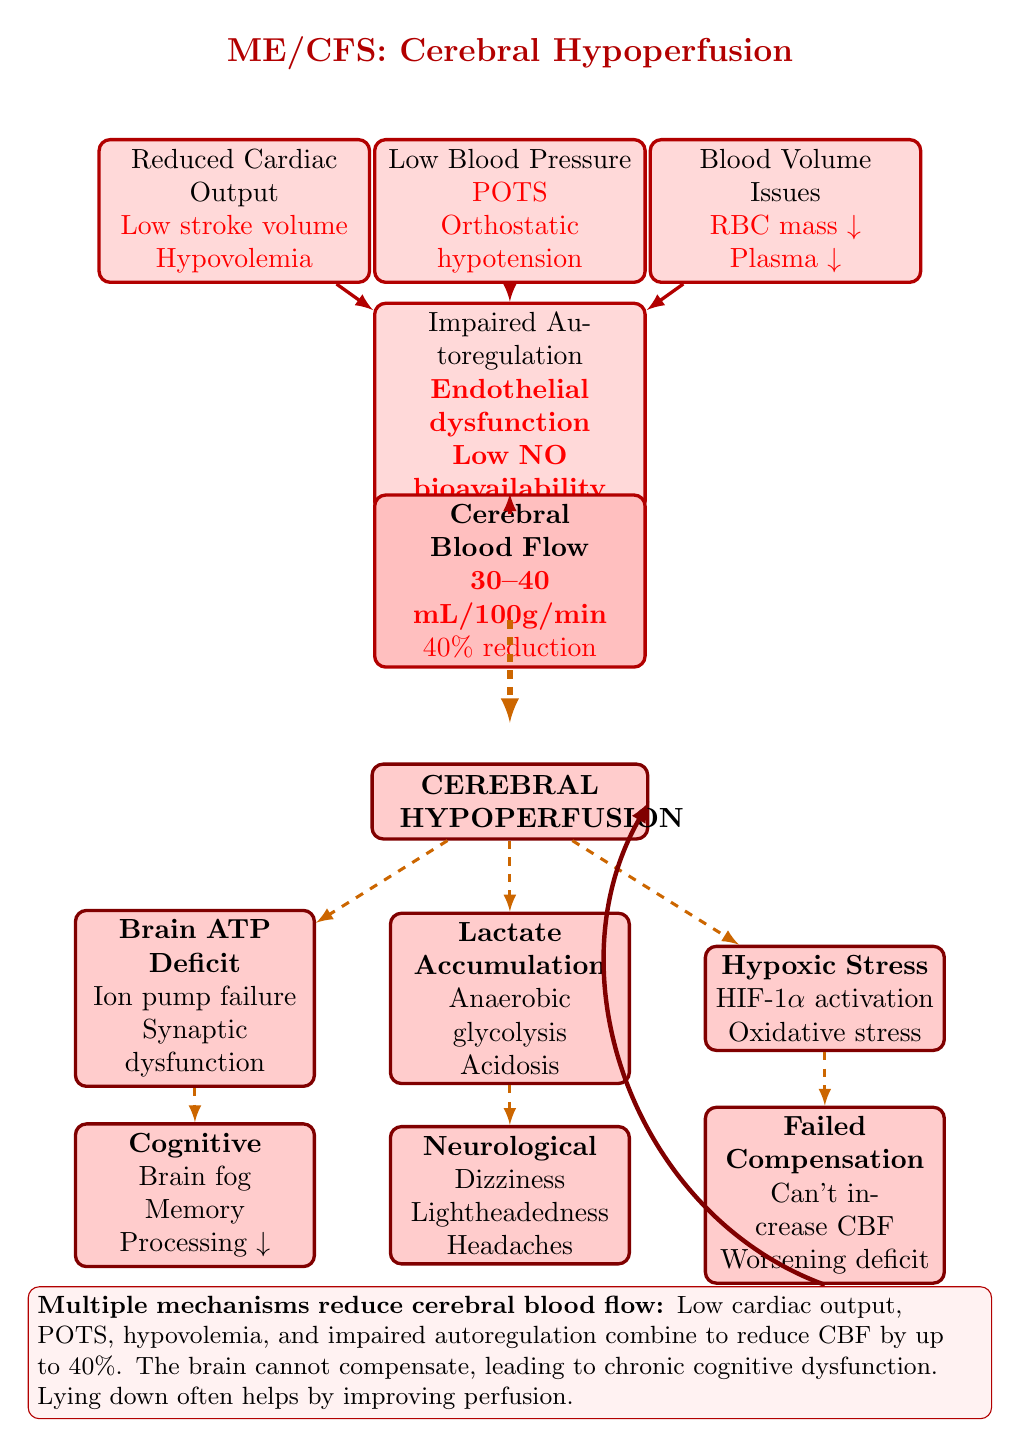
\begin{tikzpicture}[scale=1, every node/.style={scale=1},
    % Styles
    normal/.style={draw=green!70!black, fill=green!10, very thick, rounded corners, text width=3cm, align=center, minimum height=1cm},
    impaired/.style={draw=red!70!black, fill=red!15, very thick, rounded corners, text width=3.2cm, align=center, minimum height=1cm},
    severe/.style={draw=red!50!black, fill=red!25, ultra thick, rounded corners, text width=3.2cm, align=center, minimum height=1.1cm, drop shadow},
    pathological/.style={draw=red!50!black, fill=red!20, very thick, rounded corners, text width=2.8cm, align=center, minimum height=0.95cm},
    impaired-arrow/.style={-latex, very thick, red!70!black, line width=1.2pt},
    cascade-arrow/.style={-latex, thick, orange!80!black, dashed, line width=1.1pt},
    cycle-arrow/.style={-latex, ultra thick, red!50!black, line width=1.6pt},
    note/.style={font=\small\itshape, text width=2.4cm, align=left, red!60!black},
]

% Title
\node[font=\large\bfseries, red!70!black] at (0, 9) {ME/CFS: Cerebral Hypoperfusion};

% TOP: Impaired flow pathway
\begin{scope}[yshift=4.5cm]
    % Multiple contributors
    \node[impaired] (cardiac) at (-3.5, 2.5) {Reduced Cardiac\\Output\\{\color{red}Low stroke volume}\\{\color{red}Hypovolemia}};

    \node[impaired] (bp) at (0, 2.5) {Low Blood Pressure\\{\color{red}POTS}\\{\color{red}Orthostatic\\hypotension}};

    \node[impaired] (volume) at (3.5, 2.5) {Blood Volume\\Issues\\{\color{red}RBC mass $\downarrow$}\\{\color{red}Plasma $\downarrow$}};

    % Impaired autoregulation
    \node[impaired] (autoreg) at (0, 0) {Impaired Autoregulation\\{\color{red}\textbf{Endothelial dysfunction}}\\{\color{red}\textbf{Low NO bioavailability}}};
    \draw[impaired-arrow] (cardiac) -- (autoreg);
    \draw[impaired-arrow] (bp) -- (autoreg);
    \draw[impaired-arrow] (volume) -- (autoreg);

    % Reduced CBF
    \node[impaired, fill=red!25] (cbf) at (0, -2.2) {\textbf{Cerebral Blood Flow}\\{\color{red}\textbf{30--40 mL/100g/min}}\\{\color{red}40\% reduction}};
    \draw[impaired-arrow] (autoreg) -- (cbf);
\end{scope}

% BOTTOM: Cascade consequences
\begin{scope}[yshift=-3.5cm]
    % Central hypoperfusion
    \node[pathological, minimum width=3.5cm] (hypoperf) at (0, 3) {\textbf{CEREBRAL}\\  \textbf{HYPOPERFUSION}};

    % Three immediate consequences
    \node[pathological] (atp) at (-4, 0.5) {\textbf{Brain ATP}\\  \textbf{Deficit}\\Ion pump failure\\Synaptic dysfunction};

    \node[pathological] (lactate) at (0, 0.5) {\textbf{Lactate}\\  \textbf{Accumulation}\\Anaerobic glycolysis\\Acidosis};

    \node[pathological] (hypoxia) at (4, 0.5) {\textbf{Hypoxic Stress}\\HIF-1$\alpha$ activation\\Oxidative stress};

    \draw[cascade-arrow] (hypoperf) -- (atp);
    \draw[cascade-arrow] (hypoperf) -- (lactate);
    \draw[cascade-arrow] (hypoperf) -- (hypoxia);

    % Downstream symptoms
    \node[pathological] (cognitive) at (-4, -2) {\textbf{Cognitive}\\Brain fog\\Memory\\Processing $\downarrow$};

    \node[pathological] (neuro) at (0, -2) {\textbf{Neurological}\\Dizziness\\Lightheadedness\\Headaches};

    \node[pathological] (failed) at (4, -2) {\textbf{Failed}\\  \textbf{Compensation}\\Can't increase CBF\\Worsening deficit};

    \draw[cascade-arrow] (atp) -- (cognitive);
    \draw[cascade-arrow] (lactate) -- (neuro);
    \draw[cascade-arrow] (hypoxia) -- (failed);

    % Feedback loop
    \draw[cycle-arrow, bend left=50] (failed.south) to (hypoperf.east);
\end{scope}

% Arrow connecting top to bottom
\draw[cascade-arrow, line width=2pt] (0, 1.8) -- (0, 0.5);

% Key point box
\node[draw=red!70!black, fill=red!5, rounded corners, text width=12cm, align=left, font=\small] at (0, -7.5) {
\textbf{Multiple mechanisms reduce cerebral blood flow:} Low cardiac output, POTS, hypovolemia, and impaired autoregulation combine to reduce CBF by up to 40\%. The brain cannot compensate, leading to chronic cognitive dysfunction. Lying down often helps by improving perfusion.
};

\end{tikzpicture}
\caption{ME/CFS cerebral hypoperfusion cascade causing cognitive dysfunction.}
\label{fig:cerebral-hypoperfusion-mecfs}
\end{figure}


Figures~\ref{fig:cerebral-hypoperfusion-normal} and~\ref{fig:cerebral-hypoperfusion-mecfs} illustrate how multiple mechanisms reduce cerebral blood flow in ME/CFS (30--40 mL/100g/min vs.\ normal 50--60 mL/100g/min, a 40\% reduction).

\subsection{Reduced Regional Blood Flow}

Multiple neuroimaging modalities have demonstrated CBF reductions~\cite{vanCampen2020severity}:

\begin{itemize}
    \item \textbf{Global hypoperfusion}: 10--20\% reduction in total cerebral blood flow (measured by SPECT and Doppler ultrasound)
    \item \textbf{Regional deficits}: Particularly in frontal, temporal, and parietal regions
    \item \textbf{Brainstem hypoperfusion}: Potentially explaining autonomic dysfunction~\cite{Barnden2011brainstem}
    \item \textbf{Subcortical abnormalities}: Basal ganglia and thalamic hypoperfusion
\end{itemize}

Van Campen et al.~\cite{vanCampen2020severity} documented that 90\% of ME/CFS patients (n=429) showed abnormal CBF reduction (>13\%) during head-up tilt testing, with end-tilt CBF reduction of 26\% in ME/CFS patients versus only 7\% in controls (n=44). Importantly, this occurred even in the absence of hypotension or tachycardia, indicating intrinsic cerebrovascular dysfunction rather than solely cardiovascular causes.

\subsection{Correlation with Cognitive Symptoms}

CBF reductions correlate with specific cognitive deficits:

\begin{itemize}
    \item Frontal hypoperfusion → executive dysfunction, working memory impairment
    \item Temporal hypoperfusion → verbal memory deficits, language processing difficulties
    \item Parietal hypoperfusion → attention deficits, spatial processing impairment
    \item Global hypoperfusion → processing speed reduction, mental fatigue
\end{itemize}

\subsection{Mechanisms of Cerebral Hypoperfusion}

The cerebral hypoperfusion documented above likely results from multiple converging mechanisms:

\begin{itemize}
    \item \textbf{Reduced cardiac output}: Secondary to autonomic dysfunction (Section~\ref{sec:ans-pathophysiology}) and blood volume deficits~\cite{Streeten1998blood}
    \item \textbf{Impaired cerebral autoregulation}: Inability to maintain CBF across blood pressure changes~\cite{Barnden2011brainstem}
    \item \textbf{Endothelial dysfunction}: Reduced nitric oxide-mediated vasodilation
    \item \textbf{Increased cerebrovascular resistance}: Vasoconstriction or structural changes
    \item \textbf{Neurovascular uncoupling}: Failure of blood flow to match metabolic demand
\end{itemize}

The integration of autonomic dysfunction, reduced blood volume, and direct cerebrovascular pathology creates a multifactorial reduction in brain perfusion that correlates with cognitive symptom severity. This multifactorial integration is characteristic of ME/CFS pathophysiology and is discussed in the context of multi-system interactions in Chapter~\ref{ch:integrative-models}, Section~\ref{sec:synthesis}.

\subsection{Exacerbation with Exertion}

Importantly, cerebral perfusion abnormalities worsen following physical or cognitive exertion:

\begin{itemize}
    \item Further CBF reductions post-exercise
    \item Prolonged recovery of normal perfusion
    \item Correlation with post-exertional malaise severity
    \item Potential contribution to cognitive ``crashes'' following activity
\end{itemize}

\section{Auditory Processing Dysfunction and Tinnitus}
\label{sec:auditory-dysfunction}

Auditory symptoms represent an underrecognized but significant neurological manifestation of ME/CFS, with convergent evidence from functional, epidemiological, systematic, and anatomical studies establishing auditory dysfunction as a documented feature of the disease.

\subsection{Prevalence and Epidemiology}

\begin{achievement}[Tinnitus-ME/CFS Epidemiological Association]
\label{ach:schubert2021-tinnitus}
Schubert et al.~\cite{Schubert2021} provided the first large-scale epidemiological evidence linking ME/CFS to tinnitus in a population-based cohort of 124,609 individuals from the Dutch Lifelines study. ME/CFS patients demonstrated 1.57 times higher odds (OR 1.568, p<0.05) of experiencing constant tinnitus compared to healthy controls, identifying ME/CFS as a novel disease associate for tinnitus beyond traditional audiological causes such as noise exposure, age-related hearing loss, and cardiovascular disease.
\end{achievement}

This finding aligns with earlier cohort studies and patient surveys reporting tinnitus prevalence ranging from 48\% to 78\% in ME/CFS patients, substantially higher than the 10--15\% prevalence in the general population.

\begin{achievement}[Systematic Evidence for Auditory Dysfunction]
\label{ach:skare2024-ear}
A 2024 systematic review by Skare et al.~\cite{Skare2024} synthesized evidence from 172 articles (1990--2024) documenting ear abnormalities across ME/CFS, fibromyalgia, long-COVID syndrome, postural orthostatic tachycardia syndrome (PoTS), and related conditions. The review identified cochlear complaints---including tinnitus, hearing loss, and hyperacusis---as the most frequent auditory findings in ME/CFS. Four pathophysiological mechanisms were proposed: (1) viral effects on cochlear or central auditory structures, (2) vascular impairment reducing blood flow to the cochlea and brainstem, (3) autoimmune reactions targeting inner ear antigens, and (4) oxidative stress damaging cochlear hair cells and auditory neurons.
\end{achievement}

The systematic review recommended that all ME/CFS patients with audiological complaints receive ENT consultation and formal audiometry to assess the nature and severity of auditory dysfunction.

\subsection{Functional Auditory Processing Deficits}

Beyond subjective tinnitus complaints, objective evidence demonstrates specific auditory processing impairments in ME/CFS patients.

\begin{achievement}[Selective Auditory Processing Impairment]
\label{ach:johnson1996-auditory}
Johnson et al.~\cite{Johnson1996} demonstrated modality-specific cognitive impairment in a controlled comparison of 20 CFS patients, 20 multiple sclerosis (MS) patients, and 20 healthy controls. CFS patients showed differential impairment on auditory versus visual processing tasks, while MS patients showed equal impairment on both modalities. This pattern suggests specific dysfunction in central auditory pathways rather than general cognitive slowing, distinguishing the ME/CFS cognitive profile from the more global impairment observed in other neurological conditions.
\end{achievement}

Functional MRI studies have further documented that CFS patients utilize more extensive brain regions for auditory processing compared to controls, requiring greater neural recruitment and elevated source current to achieve equivalent performance. This suggests inefficient auditory processing requiring compensatory activation of additional neural networks.

\subsection{Neuroanatomical Substrate: Brainstem Dysfunction}

The functional auditory deficits and elevated tinnitus prevalence in ME/CFS are explained by documented structural and functional abnormalities in brainstem regions critical for auditory processing.

\begin{achievement}[Brainstem Structural Abnormalities]
\label{ach:nelson2021-brainstem}
Nelson et al.~\cite{Nelson2021} synthesized MRI evidence from 11 studies demonstrating structural and functional brainstem abnormalities in ME/CFS patients. The brainstem contains the primary central auditory pathway structures:

\begin{itemize}
    \item \textbf{Cochlear nucleus} (medulla) --- receives input from cochlear nerve; first central processing station
    \item \textbf{Superior olivary complex} (pons) --- sound localization via interaural time and intensity differences
    \item \textbf{Lateral lemniscus} --- ascending auditory pathway connecting lower and upper brainstem
    \item \textbf{Inferior colliculus} (midbrain) --- integration of ascending auditory information before thalamic relay
\end{itemize}

Dysfunction in these structures provides a neuroanatomical substrate explaining both the auditory processing deficits documented by Johnson et al.~\cite{Johnson1996} and the increased tinnitus prevalence observed by Schubert et al.~\cite{Schubert2021}.
\end{achievement}

Importantly, brainstem abnormalities in ME/CFS extend beyond auditory pathways to include autonomic control centers (see Section~\ref{sec:ans-pathophysiology}), arousal systems (locus coeruleus), and sensory integration regions. This explains the co-occurrence of auditory symptoms with autonomic dysfunction, sleep disturbances, and sensory hypersensitivity---all manifestations of brainstem pathology.

\subsection{Central vs. Peripheral Auditory Pathology}

\begin{observation}[Central vs. Peripheral Auditory Pathology]
\label{obs:central-auditory}
The convergence of functional deficits~\cite{Johnson1996}, population-level tinnitus prevalence~\cite{Schubert2021}, systematic evidence~\cite{Skare2024}, and brainstem MRI abnormalities~\cite{Nelson2021} suggests predominantly \textbf{central (brainstem)} rather than peripheral (cochlear) auditory pathology in ME/CFS. This distinction has important therapeutic implications: neurological approaches targeting brainstem dysfunction, cerebral perfusion, and neuroinflammation may be more effective than peripheral ENT interventions focused solely on the cochlea or middle ear.
\end{observation}

Evidence supporting central over peripheral pathology includes:

\begin{itemize}
    \item Auditory processing deficits may occur without peripheral hearing loss on audiometry
    \item Tinnitus severity often fluctuates with orthostatic stress and cerebral hypoperfusion
    \item Auditory symptoms co-occur with other brainstem-mediated dysfunction (autonomic, arousal, sensory)
    \item Hyperacusis (sound sensitivity) suggests central gain dysregulation rather than peripheral damage
    \item Auditory symptoms are part of broader post-exertional malaise rather than isolated ear pathology
\end{itemize}

\subsection{Proposed Mechanisms}

Based on the systematic review by Skare et al.~\cite{Skare2024} and integration with established ME/CFS pathophysiology, four mechanisms likely contribute to auditory dysfunction (this exemplifies the multi-mechanism pattern characteristic of ME/CFS symptoms, as discussed in Chapter~\ref{ch:integrative-models}):

\paragraph{Viral Effects.}
Direct viral damage to cochlear structures or central auditory pathways may occur during acute infection. This is particularly relevant for post-infectious ME/CFS onset, where viral neurotropism (e.g., EBV, HHV-6) could affect brainstem auditory nuclei. Acute onset of tinnitus following infection supports this mechanism.

\paragraph{Vascular Impairment.}
Reduced cerebral blood flow documented in ME/CFS (Section~\ref{sec:cerebral-blood-flow}) likely affects the highly vascularized cochlea and brainstem auditory centers. The stria vascularis in the cochlea maintains the ionic gradient essential for sound transduction and is metabolically active, making it vulnerable to hypoperfusion. Fluctuating tinnitus severity correlating with orthostatic stress supports vascular involvement.

\paragraph{Autoimmune Reactions.}
Antibodies targeting inner ear antigens (anti-cochlin, anti-HSP70) or auditory brainstem structures may produce autoimmune inner ear disease (AIED). This mechanism aligns with broader autoimmune theories of ME/CFS and suggests potential benefit from immunomodulatory treatment in select patients.

\paragraph{Oxidative Stress.}
Reactive oxygen species generated by mitochondrial dysfunction and neuroinflammation can damage cochlear hair cells and auditory neurons. The cochlea has high metabolic demands and limited antioxidant capacity, making it vulnerable to oxidative damage. This mechanism connects auditory dysfunction to the mitochondrial pathology documented in ME/CFS.

\subsection{Clinical Implications}

\subsubsection{Assessment Recommendations}

Based on the documented prevalence and clinical significance of auditory dysfunction:

\begin{enumerate}
    \item \textbf{Routine screening}: All ME/CFS patients should be screened for tinnitus, hearing loss, hyperacusis, and auditory processing difficulties
    \item \textbf{Formal audiometry}: Patients reporting auditory symptoms should receive comprehensive audiological evaluation
    \item \textbf{ENT consultation}: Rule out treatable peripheral causes (cerumen impaction, otosclerosis, Ménière's disease)
    \item \textbf{Central auditory testing}: Consider auditory brainstem response (ABR) testing to assess central pathways
    \item \textbf{Correlation with ME/CFS severity}: Document whether auditory symptoms fluctuate with overall disease activity, orthostatic stress, and post-exertional malaise
\end{enumerate}

\subsubsection{Treatment Considerations}

Given the proposed central pathology:

\begin{itemize}
    \item \textbf{Address underlying ME/CFS pathophysiology}: Optimize cerebral perfusion (salt/fluid loading for orthostatic intolerance), treat neuroinflammation, support mitochondrial function
    \item \textbf{Symptomatic management}: Sound therapy (white noise, tinnitus masking), cognitive-behavioral therapy for tinnitus distress (distinct from CBT as ME/CFS treatment)
    \item \textbf{Avoid ototoxic medications}: Many drugs can worsen tinnitus (aminoglycosides, loop diuretics, high-dose aspirin, certain chemotherapies)
    \item \textbf{Consider immunomodulation}: In patients with evidence of autoimmune component (autoantibodies, inflammatory markers)
    \item \textbf{Antioxidant support}: Alpha-lipoic acid, CoQ10, N-acetylcysteine (extrapolated from evidence in age-related hearing loss and noise-induced damage)
\end{itemize}

\begin{warning}[Tinnitus as PEM Symptom]
Many ME/CFS patients report that tinnitus intensity increases during post-exertional malaise or correlates with fatigue severity. This pattern suggests tinnitus may function as a real-time indicator of energy depletion or cerebral hypoperfusion. Patients should be educated to recognize worsening tinnitus as a potential warning sign to rest and avoid further exertion.
\end{warning}

\subsection{Research Gaps}

Despite the convergent evidence for auditory dysfunction in ME/CFS, significant gaps remain:

\begin{itemize}
    \item \textbf{Causality}: Cross-sectional designs cannot determine whether ME/CFS causes auditory dysfunction, auditory dysfunction contributes to ME/CFS symptoms, or a common mechanism produces both
    \item \textbf{Subtype correlation}: Unknown whether auditory symptoms predict specific ME/CFS subgroups or correlate with particular biomarkers
    \item \textbf{Treatment trials}: No randomized controlled trials of auditory-targeted interventions in ME/CFS populations
    \item \textbf{Mechanism validation}: The four proposed mechanisms (viral, vascular, autoimmune, oxidative) require experimental validation
    \item \textbf{Reversibility}: Unknown whether treating underlying ME/CFS pathophysiology can reverse auditory dysfunction
    \item \textbf{Longitudinal trajectory}: Natural history of auditory symptoms in ME/CFS not systematically documented
\end{itemize}

\begin{open_question}[Central Auditory Gain and Sensory Hypersensitivity]
Hyperacusis (sound sensitivity) in ME/CFS may reflect dysregulated central gain in auditory processing pathways. The brainstem and auditory cortex normally adjust sensitivity (gain) based on environmental demands and context. In ME/CFS, chronic neuroinflammation, altered neurotransmitter levels, or thalamic dysfunction may inappropriately increase central auditory gain, amplifying all sounds and making normal environmental noise intolerable. This would parallel central sensitization in pain pathways. Testing this hypothesis with objective measures of auditory gain (acoustic reflex thresholds, loudness discomfort levels, auditory brainstem response) could clarify mechanisms and guide treatment targeting central gain normalization rather than peripheral protection.
\end{open_question}

\section{Cognitive Dysfunction: Clinical Manifestations}
\label{sec:cognitive-clinical}

The neurological abnormalities described above manifest clinically as characteristic patterns of cognitive dysfunction, often described by patients as ``brain fog.''

\subsection{Domains of Impairment}

\subsubsection{Processing Speed}

Slowed information processing is perhaps the most consistent cognitive finding, manifesting as delayed reaction times, slower performance on timed tasks, reduced ability to keep up with rapid conversations, and difficulty with time-pressured activities.

\subsubsection{Attention and Concentration}

Attention and concentration deficits include difficulty sustaining attention, easy distractibility, impaired divided attention (multitasking), and reduced attentional capacity under stress.

\subsubsection{Memory}

Memory impairments encompass working memory deficits (holding information ``online''), impaired short-term memory encoding, word-finding difficulties, and variable long-term memory retrieval.

\begin{hypothesis}[Memory Triage Consequence]
\label{hyp:memory-triage-consequence}

Memory encoding is substantially more energy-expensive than memory retrieval, predicting that ME/CFS patients should show disproportionate encoding deficits relative to retrieval impairment---a pattern consistent with CNS energy triage.

\paragraph{Differential energy costs of memory operations.}
Hippocampal memory encoding requires long-term potentiation (LTP), involving NMDA receptor activation, calcium-dependent signaling cascades, new protein synthesis, and structural synaptic remodeling~\cite{Kandel2014memory}. These processes are metabolically demanding: encoding a new memory trace requires de novo gene expression, dendritic spine growth, and synaptic protein trafficking. Retrieval, by contrast, reactivates existing synaptic patterns through pattern completion in CA3 networks---a process that uses established circuits without requiring new protein synthesis or structural modification~\cite{Dudai2015consolidation}.

Quantitative estimates suggest that LTP-associated protein synthesis increases local energy consumption by 30--50\% above baseline in hippocampal neurons, whereas pattern completion during retrieval operates within normal metabolic parameters. Working memory maintenance in prefrontal cortex similarly requires sustained neuronal firing against inhibitory currents, creating continuous metabolic demand proportional to the number of items held in mind~\cite{Constantinidis2018working}.

\paragraph{Predicted pattern in ME/CFS.}
If CNS energy is limited, the brain should sacrifice high-cost encoding operations before low-cost retrieval operations---a ``memory triage.'' This predicts:

\begin{enumerate}
    \item \textbf{Encoding $>$ retrieval impairment}: Patients should show greater difficulty forming new memories than accessing old ones. Standardized testing should reveal disproportionate deficits on encoding-dependent tasks (learning new word lists, forming new associations) relative to recognition or cued recall of previously encoded material
    \item \textbf{Working memory $>$ long-term retrieval}: Sustained prefrontal firing for working memory maintenance is metabolically costly; retrieving consolidated long-term memories from distributed cortical stores is less so
    \item \textbf{Encoding degrades with exertion}: During PEM, when CNS energy deficits intensify, new memory formation should decline more steeply than the ability to recall previously consolidated information
    \item \textbf{Context-dependent encoding failure}: Encoding in metabolically demanding contexts (noisy environments, multitasking, social interaction) should fail preferentially, as these conditions compete for the limited energy budget
\end{enumerate}

\paragraph{Supporting evidence.}
The meta-analysis by Sebaiti et al.~\cite{Sebaiti2022cognitive} documents memory impairment in ME/CFS with moderate effect sizes ($g = -0.55$ to $-0.67$), but existing studies have not systematically separated encoding from retrieval. Clinical observation consistently reports that ME/CFS patients struggle more with forming new memories (``I can't take in new information'') than with accessing established knowledge (``I remember things from before I got sick''). Patients frequently describe intact recognition (``I know I've seen this before'') with impaired free recall of recently encountered material---precisely the pattern predicted by encoding-selective energy limitation.

\paragraph{Treatment implications.}
If encoding is selectively impaired by energy limitation, compensatory strategies should emphasize: (1)~reducing encoding load through external memory aids (notes, recordings, photographs) rather than relying on internal encoding; (2)~scheduling new learning during peak energy windows; (3)~using spaced repetition to distribute encoding costs across multiple low-demand sessions; (4)~leveraging recognition over recall (multiple-choice formats, visual cues) when possible.

\paragraph{Limitations.}
This hypothesis has certainty 0.55. The differential energy cost of encoding versus retrieval is well established in neuroscience, but the specific prediction of disproportionate encoding impairment in ME/CFS awaits formal testing with paradigms designed to isolate encoding from retrieval. Existing neuropsychological batteries typically conflate encoding and retrieval in composite ``memory'' scores. Confounds include attention deficits (which impair encoding indirectly), medication effects, and sleep disruption (which impairs memory consolidation independently of encoding).
\end{hypothesis}

\subsubsection{Executive Function}

Executive function deficits present as planning and organization difficulties, impaired cognitive flexibility, reduced problem-solving ability, and difficulty with complex decision-making.

\subsection{Social and Emotional Dysfunction}
\label{subsec:social-emotional-dysfunction}

While less frequently discussed in clinical literature, social and emotional impairments represent significant sources of disability in ME/CFS and are direct consequences of the neurometabolic dysfunction documented above.

\textbf{Note on evidence base:} The detailed phenomenology described in this section is based primarily on extensive clinical observation and patient reports rather than systematic empirical research. While the underlying neurobiological mechanisms (catecholamine depletion, prefrontal hypometabolism, TPJ dysfunction) are well-documented~\cite{walitt2024deep}, the specific social and emotional manifestations described below await formal validation through patient surveys, qualitative research, and prospective studies. This section should be considered a synthesis of clinical observation with established neuroscience, not yet a body of peer-reviewed ME/CFS-specific research on social disability.

\subsubsection{Social Interaction as Metabolically Demanding Activity}

Social interaction requires the simultaneous coordination of multiple high-energy cognitive and neurological processes:

\begin{itemize}
    \item \textbf{Language processing and production}: Real-time comprehension, response formulation, word retrieval, and articulation
    \item \textbf{Working memory load}: Tracking conversational context, remembering prior statements, maintaining coherent narrative threads
    \item \textbf{Executive function demands}: Monitoring social cues, adjusting behavior in real-time, inhibiting inappropriate responses
    \item \textbf{Sensory integration}: Simultaneous processing of facial expressions, vocal prosody, body language, and environmental context
    \item \textbf{Motor control for affect generation}: Voluntary and involuntary facial expressions, eye contact, postural adjustments, vocal modulation
    \item \textbf{Reward system engagement}: Dopamine-mediated reward processing that makes social interaction inherently reinforcing in healthy individuals
\end{itemize}

When ATP production is impaired and catecholamine levels are low (as documented in the NIH study~\cite{walitt2024deep}), these processes cannot be sustained. The brain experiences social demands as it would physical exertion beyond capacity: as painful, threatening, something to avoid.

\subsubsection{Clinical Presentation: Social Interaction as Painful Exertion}

Many ME/CFS patients report that social interaction feels actively \textit{painful} rather than merely tiring:

\begin{itemize}
    \item Subjective experience identical to being forced to perform physical exercise while exhausted
    \item Approach characterized by ``minimize the pain''---engage only as much as absolutely necessary
    \item Absence of enjoyment or reward, even in interactions that would previously have been pleasurable
    \item Duration often measured in minutes before exhaustion becomes overwhelming
    \item Post-social crashes (cognitive and physical PEM) lasting hours to days
\end{itemize}

This pattern may persist for decades and often predates formal ME/CFS diagnosis, suggesting it reflects fundamental metabolic limitations rather than secondary depression or psychological withdrawal.

\subsubsection{Flat Affect and Energy Conservation}

Generating and displaying emotional affect is metabolically expensive:

\begin{itemize}
    \item \textbf{Muscular activation}: Smiling, animated facial expressions, and expressive body language require continuous motor control
    \item \textbf{Neurochemical substrates}: Emotional expression requires adequate dopamine for motivation and reward signaling
    \item \textbf{Prefrontal-limbic coordination}: Generating contextually appropriate affect requires coordination between multiple brain regions
\end{itemize}

When energy is scarce, the brain prioritizes survival functions over social signaling. The result is observable flat affect---patients appear emotionally unexpressive, disengaged, or ``unhappy'' even when not experiencing negative emotion. This is \textbf{not} conscious suppression or masking; it reflects genuine inability to generate the energetic and neurochemical processes required for emotional expression.

\subsubsection{Interpersonal Consequences and Misattribution}

The combination of social withdrawal and flat affect creates predictable interpersonal difficulties:

\begin{itemize}
    \item \textbf{Misinterpretation as contempt or disinterest}: Observers lacking context for the patient's energy deficit often interpret flat affect and minimal engagement as disdain, superiority, or lack of care
    \item \textbf{Relationship damage}: Colleagues, friends, and family members feel rejected, judged, or dismissed when the actual issue is metabolic incapacity
    \item \textbf{Emotional contagion}: Others interacting with ME/CFS patients often become unhappy or uncomfortable themselves, unable to understand the patient's apparent lack of positive affect
    \item \textbf{Inability to explain}: The exhaustion that prevents social engagement also impairs the cognitive and communication capacity needed to explain the problem (``explaining why I'm too tired to talk requires energy to talk'')
    \item \textbf{Vicious cycle}: Negative reactions from others increase the stress and energy demand of social interaction, further reducing capacity
\end{itemize}

Patients are frequently blamed for ``attitude problems,'' ``not trying,'' or ``not caring'' when the actual issue is neurometabolic failure to generate expected social signals.

\subsubsection{The Communication Double-Bind}

ME/CFS patients face an impossible situation regarding social interaction:

\begin{enumerate}
    \item Employment and relationships require communication and social engagement
    \item Communication and social engagement are painfully exhausting and worsen symptoms
    \item Avoiding social interaction damages relationships and is misinterpreted as contempt
    \item Explaining the difficulty requires the very communication capacity that is depleted
    \item There is no winning strategy---only choices between different types of harm
\end{enumerate}

\subsubsection{Relationship Conflict as Insurmountable Barrier}

The energy deficit affecting social interaction becomes critically limiting when relationships encounter even minor conflict or tension:

\begin{itemize}
    \item \textbf{Conflict management requires peak cognitive resources}: Navigating disagreements, processing emotions, formulating diplomatic responses, regulating one's own reactions, and sustaining conversation through discomfort all require executive function, emotional regulation, and sustained attention---precisely the capacities most impaired in ME/CFS

    \item \textbf{Minor conflicts become insurmountable}: What healthy individuals would consider trivial relationship friction (scheduling disagreements, differing preferences, minor miscommunications) becomes \textit{impossibly difficult to manage} when cognitive and emotional resources are depleted

    \item \textbf{Relationship attrition}: Friendships require ongoing maintenance, occasional conflict resolution, and emotional investment. When any conflict---however minor---exceeds available energy, relationships deteriorate and are eventually abandoned

    \item \textbf{Selection for low-maintenance relationships only}: Only relationships requiring absolutely minimal effort, zero conflict, and no emotional complexity can be sustained. This severely restricts social connection to a vanishingly small subset of potential relationships

    \item \textbf{Inability to repair}: Even when patients recognize that a relationship is worth preserving, they lack the energy to engage in the repair conversations necessary to resolve issues. The relationship fails not from lack of desire but from metabolic inability to execute repair

    \item \textbf{Compounding isolation}: As relationships with any degree of complexity or occasional friction are abandoned due to inability to manage conflict, social networks contract to near-zero. Patients become profoundly isolated not from preference but from inability to meet the basic energy demands of relationship maintenance

    \item \textbf{Loss of deep connections}: The inability to engage seriously in friendship---to invest emotional energy, navigate normal ups and downs, work through misunderstandings---means that only the most superficial relationships can survive. Patients lose access to the deep, meaningful connections that require tolerance for occasional difficulty

    \item \textbf{Present but disengaged}: Even when patients are physically able to attend activities or gatherings, the constant underlying exhaustion limits how intensely they can engage with others. They are there in body but cannot fully participate emotionally or socially. This creates a perceptible distance that has no apparent reason---others sense the patient is ``holding back'' or ``not really there,'' but the actual cause (metabolic inability to engage more deeply) is invisible

    \item \textbf{Engagement intensity limited by energy, not desire}: The degree of warmth, enthusiasm, investment, and genuine connection patients can offer is capped by available energy, not by their feelings toward others. Friendships that would otherwise be close remain distant because the patient cannot sustain the energy for deeper engagement, creating unexplained coldness that damages the relationship despite the patient's genuine care

    \item \textbf{Inability to develop meaningful feelings}: The energy limitation affects not only the expression of feelings but the development of feelings themselves. Emotional attachment, fondness, care, and affection require sustained interaction, shared experiences, emotional investment, and cognitive processing to develop. When energy constraints prevent this sustained engagement, feelings toward others remain shallow or fail to develop beyond superficial acquaintance. Patients find themselves unable to develop the deep care and emotional connection that would normally arise in friendships, creating a profound sense of emotional emptiness and isolation even when physically surrounded by potential friends

    \item \textbf{Social interactions as potential threats}: The knowledge that any conflict or difficulty is insurmountable leads to a defensive posture where many interactions are experienced as \textit{opportunities to be aggressed}. Since patients lack the energy to manage disagreement, navigate misunderstanding, or repair relationship damage, any interaction carries the risk of creating a problem they cannot solve. This produces preventive behavior---emotional guardedness, avoidance of deeper topics, reluctance to express needs or preferences---that further impedes the ability to connect with others. Patients become hypervigilant for potential conflict and withdraw preemptively to avoid situations they cannot metabolically handle, creating a self-protective isolation that others perceive as coldness or lack of trust
\end{itemize}

\textbf{Clinical significance:} The inability to manage even minimally conflictual relationships represents a major, under-recognized source of social disability in ME/CFS. \textbf{This cannot be understated}: patients lose friendships, partnerships, and entire social networks not because relationships are unimportant to them, but because the cognitive and emotional energy required to navigate normal relationship dynamics exceeds available capacity.

The defensive stance toward social interaction---experiencing interactions as potential threats and adopting preventive behaviors---is not paranoia or social anxiety disorder. It is a rational response to genuine incapacity. When any disagreement or misunderstanding represents an insurmountable problem due to energy deficit, hypervigilance and preemptive withdrawal become adaptive survival strategies, though they further entrench isolation.

Critically, \textit{the feeling alone is sufficient to drive protective behavior}. Patients do not need to consciously analyze the risk or make deliberate decisions to withdraw---the subjective experience of interactions as threatening automatically triggers defensive responses. This emotional reality shapes behavior independent of objective threat assessment, making the social disability self-reinforcing: the feeling of vulnerability produces protective isolation, which prevents connection, which maintains isolation.

\subsubsection{Environmental Control as Survival Mechanism}

The energy deficit necessitates a level of environmental control that is incompatible with normal social spontaneity and fundamentally at odds with what others experience as ``the joy of life'':

\begin{itemize}
    \item \textbf{Need for high control}: Patients require predictability, structure, and control over their environment to prevent energy-depleting surprises. Unforeseen events, changes in plans, unexpected social demands, or environmental chaos each represent potential energy expenditures that may trigger crashes

    \item \textbf{Incompatibility with spontaneity}: What healthy individuals experience as joyful spontaneity---surprise visits, impromptu plans, playful chaos, unexpected adventures---registers for ME/CFS patients as threatening unpredictability requiring energy they do not have

    \item \textbf{Others' joy as patient's stress}: When others behave in ways they enjoy---being spontaneous, playful, or socially unpredictable---they create a more energetically demanding environment for patients. The very behaviors that make life feel vibrant and enjoyable for healthy people increase the metabolic burden and stress for patients beyond what they can afford to manage

    \item \textbf{Inability to ``let go''}: Patients cannot easily relax control over their environment because this control is \textit{almost vital} to avoid exhaustion and crashes. What appears as rigidity, controlling behavior, or inability to be spontaneous is actually a survival mechanism---without environmental control, energy expenditure becomes unpredictable and unmanageable

    \item \textbf{Social consequences}: Others perceive the need for control as rigidity, inflexibility, being ``no fun,'' or being controlling. Patients are seen as unable to enjoy life, overly cautious, or anxiety-driven when the actual issue is metabolic necessity

    \item \textbf{The paradox of joy}: Patients are often told to ``relax,'' ``let go,'' ``be spontaneous,'' or ``just have fun''---but these very behaviors require energy reserves they do not possess. The inability to engage in joyful spontaneity is not psychological resistance but physiological impossibility
\end{itemize}

\textbf{The fundamental incompatibility:} Normal social life thrives on a degree of unpredictability, spontaneity, and flexibility that ME/CFS patients cannot metabolically afford. The environmental control necessary for survival (avoiding crashes, managing energy) is experienced by others as joyless rigidity. Patients must choose between:

\begin{enumerate}
    \item Maintaining control to prevent crashes (perceived as controlling, rigid, unable to have fun)
    \item Allowing spontaneity to please others (risking energy depletion, crashes, worsening disability)
\end{enumerate}

There is no middle ground when energy reserves are this limited. The choice to maintain control is not preference or personality---it is metabolic necessity masquerading as behavioral rigidity.

\paragraph{The Energy Poverty Analogy.}
The psychological state of ME/CFS patients living with severe energy deficit is analogous to the lived experience of people in extreme financial poverty:

\begin{itemize}
    \item \textbf{Constant precariousness}: Just as very poor people live under constant financial stress knowing that any unforeseen expense---even an insignificant 20--50\euro\ debt---could trigger a cascade of catastrophic consequences (eviction, utility shutoff, inability to afford food or medical care), ME/CFS patients live under constant metabolic stress knowing that any unforeseen energy expenditure can trigger crashes that eliminate function for days, weeks, or permanently

    \item \textbf{Inability to absorb shocks}: People with financial reserves can absorb unexpected expenses without crisis. People with energy reserves can absorb unexpected demands without crashing. Those living at the edge---whether financial or metabolic---have no buffer. Every unexpected demand is a potential catastrophe

    \item \textbf{Hypervigilance as survival}: The poor must constantly monitor their finances, avoid any unnecessary spending, and maintain rigid control over their budget to prevent disaster. ME/CFS patients must constantly monitor their energy, avoid any unnecessary expenditure, and maintain rigid control over their environment to prevent crashes. Both behaviors appear as anxiety or rigidity to those with adequate resources but are rational responses to genuine scarcity

    \item \textbf{Incomprehension from the resourced}: People with financial security cannot understand why the poor seem so anxious about ``small'' expenses or why they cannot ``just relax'' about money. People with energy reserves cannot understand why ME/CFS patients seem so anxious about ``small'' demands or why they cannot ``just relax'' and be spontaneous. The invisible nature of the deficit makes the defensive behavior appear irrational

    \item \textbf{Poverty trap dynamics}: Financial poverty creates conditions that perpetuate poverty (stress impairs decision-making, lack of resources prevents investment in improvement). Energy poverty creates conditions that perpetuate energy deficit (stress depletes energy, lack of reserves prevents activities that might improve capacity). Both are self-reinforcing traps difficult to escape

    \item \textbf{Judgment and blame}: The poor are blamed for being ``too cautious,'' ``no fun,'' unable to enjoy life, overly anxious, or having a scarcity mindset. ME/CFS patients are blamed for being controlling, rigid, unable to be spontaneous, overly anxious, or having a fearful personality. In both cases, the behavior is adaptive to genuine scarcity, not a character flaw
\end{itemize}

\textbf{Clinical significance:} Understanding ME/CFS energy management through the lens of poverty economics helps clarify why patients exhibit behaviors that appear rigid or controlling to healthy observers. The ``energy poverty'' framework explains the hypervigilance, need for control, inability to tolerate unpredictability, and constant stress as rational adaptations to living at the metabolic edge. Just as telling someone in extreme financial poverty to ``stop worrying about money and have fun'' is tone-deaf and unhelpful, telling ME/CFS patients to ``relax,'' ``let go,'' or ``be spontaneous'' fundamentally misunderstands their metabolic reality.

Even when patients \textit{can} attend activities, the pervasive exhaustion creates an invisible barrier to genuine engagement. Others perceive this as emotional distance, lack of interest, or ``holding back''---but it reflects metabolic incapacity, not psychological withdrawal. The patient may desperately want to engage more warmly, more deeply, with more enthusiasm and investment, but the energy simply does not exist. This creates relationships that feel inexplicably cold or distant despite no apparent reason, as the actual limitation (energy deficit) is invisible to observers.

This pattern is distinct from social anxiety or avoidant personality disorder---patients often desperately \textit{want} connection but physiologically \textit{cannot} sustain the energy expenditure relationships require, particularly when any degree of conflict or complexity arises.

\subsubsection{Neurobiological Basis}

The social and emotional impairments described above are explained by the documented neurological abnormalities:

\begin{itemize}
    \item \textbf{Catecholamine depletion}: Low dopamine and norepinephrine impair both reward processing (making social interaction unrewarding) and the motivation to engage socially
    \item \textbf{Prefrontal hypometabolism}: Reduced energy availability in prefrontal regions impairs the executive functions required for social cognition
    \item \textbf{Effort-reward miscalculation}: TPJ dysfunction causes the brain to perceive social interaction as high-cost, low-reward activity
    \item \textbf{Cerebral hypoperfusion}: Reduced blood flow limits the brain's capacity to sustain the metabolic demands of complex social processing
    \item \textbf{ATP depletion}: Fundamental energy insufficiency makes any sustained cognitive activity painful
\end{itemize}

\subsubsection{Clinical Significance}

\begin{tcolorbox}[colback=blue!5!white,colframe=blue!75!black,title=Recognition and Validation]
Social withdrawal and flat affect in ME/CFS are \textbf{metabolic symptoms}, not personality traits, character flaws, or pure psychiatric conditions.

\textbf{For patients:} If social interaction feels painful, if you feel no enjoyment in activities that once brought pleasure, if others tell you that you seem ``unhappy'' or ``unengaged''---these are recognized manifestations of the neurometabolic dysfunction documented in ME/CFS research. This is not your fault. You are not antisocial, cold, or broken. Your brain lacks the energy and neurochemical substrates required for normal social and emotional functioning.

\textbf{For clinicians and caregivers:} Patients who appear disengaged, flat, or ``unmotivated'' for social interaction are not exhibiting ``behavioral problems.'' They are conserving severely limited energy reserves. Pressure to ``be more social'' or ``act happier'' is equivalent to demanding that someone with severe anemia run a marathon. The physiology does not support the demand.

\textbf{For researchers:} The social and emotional dysfunction in ME/CFS deserves systematic study alongside more commonly recognized cognitive domains. Validated instruments for assessing ``social exhaustion,'' ``affective energy expenditure,'' and ``interpersonal metabolic cost'' would help quantify this significant source of disability.
\end{tcolorbox}

\begin{warning}[Harmful Advice: The ``Power of Positive Thinking'']
Some clinicians, family members, friends, and caregivers, despite good intentions, offer advice to ME/CFS patients that is not only unhelpful but actively harmful and insulting:

\textbf{The harmful message:}
\begin{itemize}
    \item ``You need to be more optimistic''
    \item ``Believing you will get better will make you better''
    \item ``Your attitude is holding you back''
    \item ``The mind-body connection means positive thinking can heal you''
    \item ``You need to stop focusing on your symptoms''
\end{itemize}

\textbf{Why this is harmful:}

\begin{enumerate}
    \item \textbf{Blames the patient for their illness}: This framing implies that patients are sick because they are not trying hard enough to think positively, placing moral responsibility for a metabolic disease on the patient's psychological state

    \item \textbf{Contradicts objective evidence}: The 2024 NIH study documented measurable neurological abnormalities---low catecholamines, TPJ dysfunction, cerebral hypoperfusion, T-cell exhaustion. These are not created or maintained by ``negative thinking'' and cannot be resolved by ``optimism''

    \item \textbf{Ignores patient experience}: Decades of lived experience show that ME/CFS patients who maintain hope, who try every treatment, who remain optimistic, still worsen or remain severely ill. The disease trajectory is independent of psychological attitude

    \item \textbf{Dismissive and insulting}: Telling someone with documented metabolic dysfunction that their attitude is the problem is equivalent to telling a diabetic that believing their pancreas works will make it produce insulin. It dismisses the physiological reality of the disease

    \item \textbf{Adds psychological burden}: Patients already carry immense guilt and self-blame (``Why can't I do what I used to do? Why am I letting everyone down?''). Being told their illness persists because they are not optimistic \textit{enough} adds psychological torment to physical suffering

    \item \textbf{Prevents appropriate treatment}: When clinicians attribute symptoms to psychological factors, they fail to investigate and treat the underlying metabolic, immunological, and neurological dysfunction

    \item \textbf{Gaslighting}: This advice constitutes medical gaslighting---denying the patient's lived reality and documented physiological abnormalities in favor of a psychosomatic explanation that places blame on the patient
\end{enumerate}

\textbf{The reality:}
\begin{itemize}
    \item ME/CFS patients are not sick because they lack optimism
    \item Positive thinking does not reverse catecholamine depletion, mitochondrial dysfunction, or immune exhaustion
    \item Many patients maintain hope and optimism for \textit{decades} while their condition worsens---their attitude did not prevent deterioration
    \item The mind-body connection exists, but it does not mean that metabolic diseases can be thought away
    \item Encouraging appropriate pacing, realistic expectations, and acceptance of limitations is more therapeutic than false promises that optimism will cure metabolic dysfunction
\end{itemize}

\textbf{For clinicians:} If you find yourself telling ME/CFS patients to ``be more optimistic'' or attributing their symptoms to psychological factors, recognize that you are:
\begin{enumerate}
    \item Contradicting objective research evidence
    \item Causing psychological harm
    \item Failing to provide appropriate medical care
    \item Perpetuating the decades of medical gaslighting that has defined ME/CFS patient experience
\end{enumerate}

The appropriate clinical response is to acknowledge the physiological reality of the disease, validate the patient's experience, support symptom management and pacing, and avoid placing the burden of recovery on the patient's psychological state.
\end{warning}

\subsection{Fluctuation and Post-Exertional Cognitive Malaise}

A characteristic feature distinguishing ME/CFS cognitive dysfunction from other conditions is its marked fluctuation, including hour-to-hour and day-to-day variability, worsening with physical, cognitive, or emotional exertion, delayed deterioration (cognitive ``payback''), and improvement with rest that rarely returns to premorbid baseline.


\subsection{CNS Energy Crisis as Primary Event}
\label{sec:cns-energy-crisis}

The selective energy dysfunction hypothesis (Section~\ref{sec:selective-dysfunction}) proposes that neurological symptoms in ME/CFS reflect \emph{primary} CNS energy failure rather than downstream effects of systemic dysfunction. Several observations support this framing:

\begin{enumerate}
    \item \textbf{CNS-specific findings}: Neuroinflammation (45--199\% elevation in key regions~\cite{Nakatomi2014neuroinflammation}), catecholamine deficiency in CSF, and regional hypometabolism are documented in the CNS specifically, not as reflections of peripheral dysfunction

    \item \textbf{Preserved autonomous processes}: Hair growth, nail growth, and basic wound healing---processes that operate locally without CNS coordination---remain intact even in severe ME/CFS, arguing against global metabolic failure

    \item \textbf{Demand-response failure}: The pattern of preserved baseline function with impaired challenge response (91--100\% show abnormal CBF reduction during orthostatic challenge~\cite{Novak2022}) is consistent with a CNS coordination bottleneck rather than peripheral end-organ dysfunction

    \item \textbf{Cognitive triage hierarchy}: The observation that complex cognition and executive function (``brain fog'') are affected before motor coordination or sensory processing suggests an energy triage system that sacrifices ``luxury'' cognitive functions first

    \item \textbf{Astrocyte vulnerability}: The brain's unique metabolic architecture---with neurons depending on astrocytes for lactate via the ANLS (Section~\ref{sec:astrocyte-energy-gate})---may create CNS-specific vulnerability not present in peripheral tissues with direct glucose access~\cite{Pellerin1994,Magistretti2018}
\end{enumerate}

This perspective has treatment implications: interventions that bypass CNS coordination (e.g., direct-acting autonomic agents like midodrine) or that specifically target CNS metabolism may be more effective than peripheral mitochondrial support alone.

\subsection{CNS Energy Triage: A Hierarchical Model of Brain Fog}
\label{sec:cns-energy-triage-clinical}

\begin{speculation}[CNS Energy Triage Hypothesis]
\label{spec:cns-energy-triage}
The brain may operate a hardwired energy prioritization system during metabolic scarcity, explaining why ME/CFS cognitive dysfunction follows a characteristic pattern rather than producing uniform degradation across all domains.

\paragraph{Neuroscience of brain energy prioritization.}
The human brain comprises approximately 2\% of body mass yet consumes 20--25\% of resting metabolic energy, with goal-directed cognition requiring only an additional $\sim$5\% above resting homeostatic costs~\cite{Jamadar2025metabolic}. This tight energy budget means that even modest metabolic deficits---such as those produced by impaired astrocyte-neuron lactate shuttling (Section~\ref{sec:astrocyte-energy-gate})---could disproportionately affect the most energy-intensive neural processes.

Not all brain regions have equal metabolic demands. The prefrontal and frontoparietal association cortices, which support executive function, cognitive flexibility, and novel problem-solving, exhibit the highest \emph{relative metabolic cost}---defined as energy utilization exceeding baseline activity levels~\cite{Jamadar2025metabolic}. In contrast, brainstem nuclei governing vital functions (respiration, cardiovascular regulation, arousal) and primary sensory cortices operate with lower relative metabolic overhead, relying on phylogenetically older, more energy-efficient circuits.

\paragraph{Evidence from metabolic disruption models.}
Two natural experiments demonstrate hierarchical cognitive shutdown under energy scarcity:

\begin{enumerate}
    \item \textbf{Hypoglycemia:} Acute reduction in brain glucose supply impairs complex higher-order cognitive processes at higher glucose thresholds and to a greater extent than lower-level functions. Executive functions show large effect sizes ($d > 0.8$) during hypoglycemia~\cite{Graveling2013hypoglycemia}, consistent with the prefrontal cortex's elevated metabolic sensitivity.

    \item \textbf{Anesthesia:} General anesthetics produce a hierarchical disconnection pattern in which prefrontal and association cortices are affected first, while primary sensory processing and thalamocortical connectivity remain preserved. Mashour characterizes this as preferential failure of ``rich club'' network hubs with greater metabolic demands~\cite{Mashour2024anesthesia}---an ``airport in a snowstorm'' analogy where the most connected, most metabolically expensive nodes fail first.
\end{enumerate}

Furthermore, prolonged cognitive work causes glutamate accumulation specifically in the lateral prefrontal cortex, making further executive function activation progressively more metabolically costly~\cite{Wiehler2022glutamate}. This suggests a built-in mechanism by which the brain curtails its most expensive operations when metabolic capacity is strained.

\paragraph{Application to ME/CFS.}
We speculate that ME/CFS produces a chronic version of this triage state. If total available CNS energy is reduced---whether through astrocyte dysfunction, reduced cerebral blood flow, or neuroinflammation---the brain may engage the same prioritization hierarchy that normally activates only during acute metabolic crises. The proposed triage order, from most to least protected, would be:

\begin{enumerate}
    \item Brainstem vital functions (preserved even in severe ME/CFS)
    \item Basic sensory processing (usually intact)
    \item Language comprehension (impaired only in severe cases)
    \item Motor coordination (degraded in moderate-severe disease)
    \item Memory consolidation (commonly affected)
    \item Executive function and cognitive flexibility (affected early, often prominently)
\end{enumerate}

This maps to the formal energy triage hypothesis developed in Section~\ref{sec:selective-dysfunction} (specifically Hypothesis~\ref{hyp:energy-triage}), but here we emphasize the clinical neuroscience basis rather than the mathematical framework.

\paragraph{An important caveat from meta-analytic evidence.}
The largest meta-analysis of cognitive impairment in ME/CFS (33 studies, $n = 1{,}086$) reveals that the observed pattern is more nuanced than a simple ``executive function fails first'' model~\cite{Sebaiti2022cognitive}. Processing speed shows the largest impairment ($g = -0.82$), followed by sustained attention ($g = -0.75$), then memory domains ($g = -0.55$ to $-0.67$), with executive function showing a smaller effect ($g = 0.42$) and instrumental functions preserved. This is important: processing speed is \emph{more} impaired than executive function on standard neuropsychological measures.

This apparent discrepancy may be reconciled by recognizing that processing speed is a \emph{global} measure of neural efficiency degraded by any reduction in brain energy delivery, not a specific cognitive tier. It reflects the overall metabolic throughput of cortical circuits rather than a discrete cognitive function. Additionally, standardized tests of executive function (e.g., Trail Making Test Part B) involve relatively routinized operations that may not capture the full metabolic cost of genuinely novel, unstructured problem-solving. The energy triage model predicts that \emph{novel, complex, integrative} cognitive operations fail first---not necessarily the specific neuropsychological domain labeled ``executive function'' in test batteries.

\paragraph{Testable predictions.}
If the CNS energy triage model is correct, the following should hold:
\begin{itemize}
    \item Novel tasks are impaired more than practiced routines at matched difficulty
    \item Working memory (high-energy encoding) fails before recognition memory (lower-energy pattern completion), as formalized in Hypothesis~\ref{hyp:memory-triage}
    \item Cognitive hierarchy of impairment maps to regional metabolic demand on FDG-PET
    \item Severity progression follows the triage order: mild ME/CFS shows primarily executive/speed deficits; severe ME/CFS additionally shows language and motor involvement
    \item Interventions that bypass energy-expensive processing (routinization, external cognitive scaffolding) should preferentially improve function
\end{itemize}

\paragraph{Treatment implications.}
If the brain operates in chronic triage mode, the therapeutic strategy shifts from ``try harder'' to ``reduce the load'': (1)~\emph{routinize} daily activities to shift them from energy-expensive prefrontal control to energy-efficient basal ganglia automaticity; (2)~use external cognitive scaffolding (lists, alarms, decision templates) to offload executive demands; (3)~schedule cognitively demanding tasks during peak energy windows when triage thresholds are temporarily relaxed; (4)~explore metabolic interventions (ketone supplementation, cerebral blood flow optimization) that may expand the total energy budget and raise triage thresholds across all tiers.

\paragraph{Limitations.}
This hypothesis faces several challenges: (1)~the meta-analytic evidence does not cleanly support executive function as the most impaired domain~\cite{Sebaiti2022cognitive}; (2)~the triage hierarchy has not been directly tested in ME/CFS with tasks specifically designed to probe each tier; (3)~alternative explanations for the cognitive pattern exist, including neuroinflammation-mediated cytokine effects on specific circuits~\cite{Bansal2025cognitive}, tryptophan pathway diversion, and autonomic-mediated cerebral hypoperfusion; (4)~the model may oversimplify what is likely a multi-mechanism process. The triage framework should be understood as one contributing mechanism among several, not a complete explanation for ME/CFS cognitive dysfunction.
\end{speculation}

\section{Summary: An Integrated Neurological Model}
\label{sec:neuro-summary}

The evidence from the NIH deep phenotyping study and decades of prior research supports an integrated model of neurological dysfunction in ME/CFS~\cite{walitt2024deep}. An initiating trigger such as infection or other stressor disrupts central nervous system homeostasis. Microglial activation persists beyond acute illness, producing chronic low-grade neuroinflammation. Catecholamine and tryptophan pathway abnormalities develop, affecting dopamine, norepinephrine, and serotonin signaling (neurotransmitter dysregulation). The temporal-parietal junction and related regions fail to accurately process effort-related information (integrative brain dysfunction). Parasympathetic withdrawal and sympathetic dysregulation produce cardiovascular and multi-organ effects (autonomic dysfunction). Reduced cerebral blood flow limits brain metabolic capacity (cerebrovascular compromise). Finally, fatigue, cognitive dysfunction, orthostatic intolerance, and other symptoms emerge from these converging abnormalities as the clinical manifestations.

This model explains why ME/CFS patients experience fatigue fundamentally different from normal tiredness: the brain's basic mechanisms for perceiving, estimating, and responding to effort are dysfunctional. Treatment approaches targeting these specific neurological abnormalities may prove more effective than those addressing peripheral fatigue or deconditioning.

\begin{warning}[Stimulant Contraindication]
Stimulants (amphetamines, methylphenidate, modafinil) are generally \textbf{contraindicated} in ME/CFS despite their effectiveness in other fatigue conditions. While they may temporarily mask fatigue by artificially boosting alertness and motivation, they do not address the underlying energy deficit and may enable activity levels that exceed the patient's true physiological capacity. This can precipitate post-exertional malaise (PEM) and potentially cause permanent deterioration. The neurological model presented here explains why: stimulants affect perceived effort and motivation (downstream of the TPJ dysfunction) without correcting the fundamental mismatch between the brain's effort calculations and actual metabolic capacity. Patients may feel capable of activity that their bodies cannot sustain, leading to crashes. This differs fundamentally from stimulant use in conditions like ADHD or narcolepsy, where the underlying metabolic machinery is intact.
\end{warning}
